% Options for packages loaded elsewhere
\PassOptionsToPackage{unicode}{hyperref}
\PassOptionsToPackage{hyphens}{url}
\PassOptionsToPackage{dvipsnames,svgnames,x11names}{xcolor}
%
\documentclass[
  12pt,
]{article}

\usepackage{amsmath,amssymb}
\usepackage{iftex}
\ifPDFTeX
  \usepackage[T1]{fontenc}
  \usepackage[utf8]{inputenc}
  \usepackage{textcomp} % provide euro and other symbols
\else % if luatex or xetex
  \usepackage{unicode-math}
  \defaultfontfeatures{Scale=MatchLowercase}
  \defaultfontfeatures[\rmfamily]{Ligatures=TeX,Scale=1}
\fi
\usepackage{lmodern}
\ifPDFTeX\else  
    % xetex/luatex font selection
\fi
% Use upquote if available, for straight quotes in verbatim environments
\IfFileExists{upquote.sty}{\usepackage{upquote}}{}
\IfFileExists{microtype.sty}{% use microtype if available
  \usepackage[]{microtype}
  \UseMicrotypeSet[protrusion]{basicmath} % disable protrusion for tt fonts
}{}
\makeatletter
\@ifundefined{KOMAClassName}{% if non-KOMA class
  \IfFileExists{parskip.sty}{%
    \usepackage{parskip}
  }{% else
    \setlength{\parindent}{0pt}
    \setlength{\parskip}{6pt plus 2pt minus 1pt}}
}{% if KOMA class
  \KOMAoptions{parskip=half}}
\makeatother
\usepackage{xcolor}
\usepackage[margin=1in]{geometry}
\setlength{\emergencystretch}{3em} % prevent overfull lines
\setcounter{secnumdepth}{-\maxdimen} % remove section numbering
% Make \paragraph and \subparagraph free-standing
\ifx\paragraph\undefined\else
  \let\oldparagraph\paragraph
  \renewcommand{\paragraph}[1]{\oldparagraph{#1}\mbox{}}
\fi
\ifx\subparagraph\undefined\else
  \let\oldsubparagraph\subparagraph
  \renewcommand{\subparagraph}[1]{\oldsubparagraph{#1}\mbox{}}
\fi


\providecommand{\tightlist}{%
  \setlength{\itemsep}{0pt}\setlength{\parskip}{0pt}}\usepackage{longtable,booktabs,array}
\usepackage{calc} % for calculating minipage widths
% Correct order of tables after \paragraph or \subparagraph
\usepackage{etoolbox}
\makeatletter
\patchcmd\longtable{\par}{\if@noskipsec\mbox{}\fi\par}{}{}
\makeatother
% Allow footnotes in longtable head/foot
\IfFileExists{footnotehyper.sty}{\usepackage{footnotehyper}}{\usepackage{footnote}}
\makesavenoteenv{longtable}
\usepackage{graphicx}
\makeatletter
\def\maxwidth{\ifdim\Gin@nat@width>\linewidth\linewidth\else\Gin@nat@width\fi}
\def\maxheight{\ifdim\Gin@nat@height>\textheight\textheight\else\Gin@nat@height\fi}
\makeatother
% Scale images if necessary, so that they will not overflow the page
% margins by default, and it is still possible to overwrite the defaults
% using explicit options in \includegraphics[width, height, ...]{}
\setkeys{Gin}{width=\maxwidth,height=\maxheight,keepaspectratio}
% Set default figure placement to htbp
\makeatletter
\def\fps@figure{htbp}
\makeatother
% definitions for citeproc citations
\NewDocumentCommand\citeproctext{}{}
\NewDocumentCommand\citeproc{mm}{%
  \begingroup\def\citeproctext{#2}\cite{#1}\endgroup}
\makeatletter
 % allow citations to break across lines
 \let\@cite@ofmt\@firstofone
 % avoid brackets around text for \cite:
 \def\@biblabel#1{}
 \def\@cite#1#2{{#1\if@tempswa , #2\fi}}
\makeatother
\newlength{\cslhangindent}
\setlength{\cslhangindent}{1.5em}
\newlength{\csllabelwidth}
\setlength{\csllabelwidth}{3em}
\newenvironment{CSLReferences}[2] % #1 hanging-indent, #2 entry-spacing
 {\begin{list}{}{%
  \setlength{\itemindent}{0pt}
  \setlength{\leftmargin}{0pt}
  \setlength{\parsep}{0pt}
  % turn on hanging indent if param 1 is 1
  \ifodd #1
   \setlength{\leftmargin}{\cslhangindent}
   \setlength{\itemindent}{-1\cslhangindent}
  \fi
  % set entry spacing
  \setlength{\itemsep}{#2\baselineskip}}}
 {\end{list}}
\usepackage{calc}
\newcommand{\CSLBlock}[1]{\hfill\break\parbox[t]{\linewidth}{\strut\ignorespaces#1\strut}}
\newcommand{\CSLLeftMargin}[1]{\parbox[t]{\csllabelwidth}{\strut#1\strut}}
\newcommand{\CSLRightInline}[1]{\parbox[t]{\linewidth - \csllabelwidth}{\strut#1\strut}}
\newcommand{\CSLIndent}[1]{\hspace{\cslhangindent}#1}

\usepackage{setspace}
\doublespacing
\makeatletter
\@ifpackageloaded{caption}{}{\usepackage{caption}}
\AtBeginDocument{%
\ifdefined\contentsname
  \renewcommand*\contentsname{Table of contents}
\else
  \newcommand\contentsname{Table of contents}
\fi
\ifdefined\listfigurename
  \renewcommand*\listfigurename{List of Figures}
\else
  \newcommand\listfigurename{List of Figures}
\fi
\ifdefined\listtablename
  \renewcommand*\listtablename{List of Tables}
\else
  \newcommand\listtablename{List of Tables}
\fi
\ifdefined\figurename
  \renewcommand*\figurename{Figure}
\else
  \newcommand\figurename{Figure}
\fi
\ifdefined\tablename
  \renewcommand*\tablename{Table}
\else
  \newcommand\tablename{Table}
\fi
}
\@ifpackageloaded{float}{}{\usepackage{float}}
\floatstyle{ruled}
\@ifundefined{c@chapter}{\newfloat{codelisting}{h}{lop}}{\newfloat{codelisting}{h}{lop}[chapter]}
\floatname{codelisting}{Listing}
\newcommand*\listoflistings{\listof{codelisting}{List of Listings}}
\makeatother
\makeatletter
\makeatother
\makeatletter
\@ifpackageloaded{caption}{}{\usepackage{caption}}
\@ifpackageloaded{subcaption}{}{\usepackage{subcaption}}
\makeatother
\ifLuaTeX
  \usepackage{selnolig}  % disable illegal ligatures
\fi
\usepackage{bookmark}

\IfFileExists{xurl.sty}{\usepackage{xurl}}{} % add URL line breaks if available
\urlstyle{same} % disable monospaced font for URLs
\hypersetup{
  pdfauthor={Steven Miles Kerr},
  colorlinks=true,
  linkcolor={blue},
  filecolor={Maroon},
  citecolor={Blue},
  urlcolor={Blue},
  pdfcreator={LaTeX via pandoc}}

\author{Steven Miles Kerr}
\date{29 April 2024}

\begin{document}

\begin{titlepage}
    \centering
    
\includegraphics[width=0.75\textwidth]{images/hertie-school-logo.jpg}
    \vspace*{\fill}
    
    \textbf{From Clicks to Cases: Leveraging Wikipedia Pageviews to Predict Mpox Cases in the United States}

    \vspace{2.5cm}

    Steven Miles Kerr

    \vspace{1cm}
    
    Master of Data Science for Public Policy, Class of 2024\\
    
    \vspace{0.5cm}

    April 29, 2024\\

    \vspace*{\fill}

    Supervised by Prof. Dr. Simon Munzert

\end{titlepage}

\tableofcontents
\thispagestyle{empty}
\newpage

\setcounter{page}{1}

\section{Abstract}\label{abstract}

As the world becomes increasingly interconnected and climate change
elevates the risk of zoonotic spillover events, the public becomes ever
more susceptible to global-scale outbreaks. Traditional disease
surveillance methods are prone to under-reporting and time lags. By
contrast, Wikipedia pageviews offer a real-time and cost-effective open
source resource for tracking online health-related information-seeking
behavior with the potential for enhancing global disease surveillance.
This paper investigates the value of anonymized country-level Wikipedia
pageviews data for predicting case incidence during the 2022-2024 mpox
outbreak in the United States. The methods employed in this study
involve a combination of quantitative techniques aimed at increasing
understanding of the relationship between online behaviors and disease
dynamics. A lag analysis correlating mpox cases and pageviews for
mpox-related Wikipedia articles at different time lags was conducted to
assess the variation in directionality between pageviews and cases
across mpox-related articles. This was followed by a multivariate linear
regression analysis aimed at predicting mpox incidence based on pageview
data. Finally, impulse response and Granger-causality tests were
performed to further analyze the directionality of the relationship
between online activity and mpox cases. The study's findings underscore
the potential of Wikipedia traffic as a predictive tool for public
health trends, revealing a bidirectional relationship between pageviews
and mpox cases that unfolds over time. The predictive models struggled
with accuracy, highlighting the need for further model refinement to
adequately account for the complexity of online attention and disease
dynamics.

\section{Introduction}\label{introduction}

As the world becomes increasingly interconnected and climate change
elevates the risk of zoonotic spillover events, the public becomes ever
more susceptible to global-scale outbreaks
(\citeproc{ref-romanello2021}{Romanello et al. 2021}). While generally
accurate, traditional surveillance methods often suffer from
under-reporting and significant time lags. In this context, such methods
are ill-equipped to provide decision-makers with real-time information
on case incidence during public health emergencies. In contrast, the
advent of data on internet activity offers an underutilized but valuable
tool for tracking health-related information-seeking behaviors. These
digital tools help bridge the gap between the occurrence of an outbreak
and its reporting, providing a more immediate picture of public health
trends and potentially accelerating policy interventions during critical
early stages of disease spread.

Google Trends serves as one such tool for analyzing global search
patterns, providing insights into public interest across countries. This
tool capitalizes on the immense traffic Google receives to evaluate the
popularity of specific keywords over time, measured by Relative Search
Volumes (RSVs). Its ability to offer real-time data on user search
behavior at no cost has made Google Trends a crucial resource in
academic research, including in the field of public health. Google Flu
Trends is perhaps the most widely recognized use case, demonstrating its
ability to produce highly accurate predictions in near real-time
(\citeproc{ref-ginsberg2009}{Ginsberg et al. 2009}). Although the
accuracy of its forecasts were compromised by factors like media
influence during particularly severe outbreaks, as seen during the 2009
H1N1 pandemic and the severe 2012-2013 flu season, it succeeded in
inspiring others to explore these methods as well
(\citeproc{ref-olson2013}{Olson et al. 2013};
\citeproc{ref-butler2013}{Butler 2013}). Researchers have demonstrated
its utility in predicting cases of diseases such as COVID-19
(\citeproc{ref-abbas2021}{Abbas et al. 2021};
\citeproc{ref-effenberger2020}{Effenberger et al. 2020};
\citeproc{ref-gong2022}{Gong et al. 2022}), malaria
(\citeproc{ref-ocampo2013}{Ocampo, Chunara, and Brownstein 2013}),
norovirus (\citeproc{ref-yuan2021}{K. Yuan et al. 2021}), and the
West-Nile virus disease (\citeproc{ref-bragazzi2016}{Bragazzi et al.
2016}) among other diseases, highlighting its potential for early
outbreak detection and public health surveillance.

While Google Trends has proven to be a powerful data source for making
case predictions, researchers have also investigated alternative data
sources including Baidu (\citeproc{ref-bao2013}{Bao et al. 2013};
\citeproc{ref-gong2022}{Gong et al. 2022}; \citeproc{ref-yuan2013}{Q.
Yuan et al. 2013}; \citeproc{ref-zhou2010}{Zhou and Shen 2010}), Reddit
(\citeproc{ref-liu2022}{Liu, Yue, and Anwar 2022}), Wikipedia
(\citeproc{ref-gozzi2020}{Gozzi et al. 2020};
\citeproc{ref-hickmann2015}{Hickmann et al. 2015};
\citeproc{ref-laurent2009}{Laurent and Vickers 2009};
\citeproc{ref-mciver2014}{McIver and Brownstein 2014};
\citeproc{ref-tausczik2012}{Tausczik et al. 2012}), and X (formerly
Twitter) (\citeproc{ref-marques-toledo2017}{Marques-Toledo et al. 2017};
\citeproc{ref-paul2011}{Paul and Dredze 2011}). Due to its freely
accessible and highly-granular pageview data, broad coverage of public
health topics, and wide readership, Wikipedia stands out as a
high-potential datastream for outbreak detection and case prediction.
While researchers have analyzed the effectiveness of Wikipedia pageview
data in the context of influenza (\citeproc{ref-hickmann2015}{Hickmann
et al. 2015}; \citeproc{ref-mciver2014}{McIver and Brownstein 2014};
\citeproc{ref-tausczik2012}{Tausczik et al. 2012}) and COVID-19
(\citeproc{ref-chrzanowski2021}{Chrzanowski et al. 2021};
\citeproc{ref-gozzi2020}{Gozzi et al. 2020}) among other diseases,
results have been mixed and have been shown to depend on the context to
which they are applied. To expand on this work and gain a better
understanding of the conditions under which Wikipedia pageview data can
be useful for making such case predictions, this paper examines the
efficacy of Wikipedia pageview data in the context of the 2022-2024 mpox
(formerly known as monkeypox) outbreak.

Mpox is a viral zoonosis---a virus transmitted to humans from
animals---with symptoms similar to those observed in smallpox patients
though typically less severe (\citeproc{ref-worldhealthorganization}{WHO
2023a}). The monkeypox virus originates from wild animals like rodents
and primates, and is spread through close contact with an infected
person or animal, or with contaminated materials
(\citeproc{ref-gessainantoine2022}{Gessain, Nakoune, and Yazdanpanah
2022}). Human symptoms of mpox include fever, rash, and swollen lymph
nodes Beer and Rao (\citeproc{ref-beer2019}{2019}). Historically, mpox
cases have been mainly reported in rural areas of western and central
Africa, with the occasional exportation to countries outside the region
(\citeproc{ref-gessainantoine2022}{Gessain, Nakoune, and Yazdanpanah
2022}).

In May 2022, multiple countries without any history of sustained local
mpox transmission reported new cases, marking the onset of a large-scale
global outbreak, prompting the World Health Organization (WHO) to
declare it a Public Health Emergency of International Concern (PHEIC) on
July 23, 2022 (\citeproc{ref-whodire}{WHO 2022b},
\citeproc{ref-secondm}{2022a}). As of March 2024, the outbreak has led
to 95,226 confirmed cases and 185 deaths across 117 countries, primarily
impacting the men who have sex with men (MSM) community
(\citeproc{ref-laurenson-schafer2023}{Laurenson-Schafer et al. 2023}).
While the emergency status was officially ended on May 11, 2023,
non-endemic countries have continued to report cases
(\citeproc{ref-fifthme}{WHO 2023c}).

Although mpox cases have been reported globally, this study specifically
examines the mpox outbreak in the United States. There are a few reasons
for this. First, the United States has reported, by far, the most mpox
cases of any country during the outbreak with a total of 32,063 cases
reported as of March 2024, comprising 33.7\% of global cases (32,063 /
95,227) (\citeproc{ref-cdc2023}{CDC 2023}; \citeproc{ref-whoshiny}{WHO
2024}). Second, the United States also has the most granular Wikipedia
pageview statistics, for reasons which will be discussed in further
detail below. For these reasons, the United States represents a
reasonable case study of the dynamic between mpox cases and Wikipedia
pageviews.

\begin{figure}[H]

{\centering \includegraphics{images/cases-USA-map.png}

}

\caption{Map of mpox cases by U.S. state}

\end{figure}%

Given the existing literature, this paper aims to fill the research gap
by investigating whether Wikipedia anonymized country-level pageview
data can be predictive of mpox cases during the 2022-2024 outbreak in
the United States. While previous studies have evaluated Wikipedia data
for COVID-19 and others have utilized Google Trends data for mpox, this
thesis represents the first attempt, to my knowledge, to explore the
relationship between Wikipedia pageview statistics and mpox cases.

\section{Literature Review}\label{literature-review}

\subsection{Public Attention}\label{public-attention}

While initially conceived outside of the field of epidemiology, Downs'
``issue-attention cycle'' can be used when analyzing public attention
toward public health emergencies. In this context, the first stage of
public attention might involve the emergency of an infectious disease
that is not recognized as a significant issue by the public
(\citeproc{ref-downs}{Downs 1972}). It may be affecting a small subset
of the population, and there may be limited awareness outside of health
professionals or those directly affected. Then, due to a rapid increase
in cases or media coverage, the public becomes highly aware of the
disease outbreak. This stage is marked by a surge in media reports and
public discussions. Over time, even as the disease continues to pose a
threat, public attention starts to decline. This could be due to a
variety of factors such as a decrease in new cases that leads to a
perception that the situation is improving, or simply desensitization to
the threat. Other emerging issues may also start drawing public and
media focus away from the outbreak. Finally, the disease may still exist
and with flare-ups occasionally occurring, but it no longer occupies
substantial public concern (\citeproc{ref-downs}{Downs 1972}).

\subsection{Digital Epidemiological
Surveillance}\label{digital-epidemiological-surveillance}

Traditional disease surveillance methods are primarily rooted in
collecting data from clinical settings such as hospitals, laboratories,
and clinics. This data often includes information on clinical diagnoses,
symptoms consistent with specific illnesses, or the number of emergency
room visits, school and work absenteeism, and other health-related
indicators (\citeproc{ref-kman2012}{Kman and Bachmann 2012}). However,
while traditional surveillance systems are crucial for accurate disease
monitoring, they have inherent limitations such as high operational
costs and significant delays in data reporting, which can extend up to
two weeks. This latency in data availability can impede timely public
health interventions, especially during urgent outbreaks.

Over the past decade, new surveillance techniques that leverage social
media and internet search data have become increasingly prominent,
offering advantages like cost-effective data collection and real-time
analysis that enhance traditional surveillance methods. These methods
consist of analyzing digital traces left by individuals discussing
health-related topics on social platforms or searching for medical
information online (\citeproc{ref-marques-toledo2017}{Marques-Toledo et
al. 2017}; \citeproc{ref-generous2014}{Generous et al. 2014}). As
internet usage continues to increase globally, this data source will
continue to benefit public health officials seeking to make informed and
data-driven policy decisions (\citeproc{ref-ginsberg2009}{Ginsberg et
al. 2009}).

\subsection{Google Trends Index}\label{google-trends-index}

Google Trends is an influential online tool that allows users to examine
global search trends, leveraging Google's status as the world's top
website (\citeproc{ref-arora2019}{Arora, McKee, and Stuckler 2019};
\citeproc{ref-topwebs}{Semrush 2024}). It offers insights into the
popularity of specific keywords over time through Relative Search
Volumes (RSVs), where a score of 100 indicates peak popularity. This
makes the Google Trends Index (GTI) a valuable resource in
epidemiological research and forecasting, such as with Google Flu Trends
which, despite its initial success in predicting flu activity in
real-time, faced accuracy challenges during major outbreaks like the
2009 H1N1 pandemic due to skewed data from media coverage
(\citeproc{ref-ginsberg2009}{Ginsberg et al. 2009};
\citeproc{ref-olson2013}{Olson et al. 2013};
\citeproc{ref-butler2013}{Butler 2013}). The tool's utility extends
beyond influenza, aiding in the forecasting of diseases like COVID-19
(\citeproc{ref-abbas2021}{Abbas et al. 2021}) and norovirus
(\citeproc{ref-yuan2021}{K. Yuan et al. 2021}) by correlating search
trends with case data.

However, Google Trends has significant limitations that affect its
practical application. It normalizes search data by assigning a score of
100 to the term's peak popularity, complicating comparisons across
different regions and times. The data resolution is limited, offering
only the most recent 90 days on a daily basis and older data weekly,
which restricts detailed long-term analysis. The lack of transparency in
Google's normalization methods and the potential for algorithm changes
introduces uncertainty and bias, potentially undermining the reliability
of longitudinal studies (\citeproc{ref-lazer2014}{Lazer et al. 2014}).

\subsection{Alternative Data Sources}\label{alternative-data-sources}

In light of Google Trends' shortcomings, researchers have explored how
other more granular data sources might be leveraged. Gong et al.~used
the Baidu Index to link COVID-19 public attention to new case
occurrences (\citeproc{ref-gong2022}{Gong et al. 2022}), while Bao et
al.~developed a predictive model for gonorrhea based on Baidu search
trends (\citeproc{ref-bao2013}{Bao et al. 2013}). Additionally, Zhou et
al.~utilized Baidu search data to forecast infection rates for diseases
like scarlet fever ahead of official statistics
(\citeproc{ref-zhou2010}{Zhou and Shen 2010}) and Yuan et al.~further
investigated the use of Baidu data through their prediction of influenza
activity in China with a mean absolute percent error under 11\% for
one-month ahead predictions (\citeproc{ref-yuan2013}{Q. Yuan et al.
2013}). Using X data on tweets, Marques-Toledo et al.~found X data could
predict dengue cases up to eight weeks ahead of official statistics
(\citeproc{ref-marques-toledo2017}{Marques-Toledo et al. 2017}).
Furthermore, Paul and Dredze built a machine learning model that
analyzed tweets for health-related topics, finding correlations with
CDC's ILI data (\citeproc{ref-paul2011}{Paul and Dredze 2011}). These
studies underscore the potential of alternative internet search engines
and social media platforms to serve as real-time surveillance tools for
anticipating and responding to public health threats.

\subsection{Wikipedia Pageviews}\label{wikipedia-pageviews}

Wikipedia is the most expansive and widely used online encyclopedia. As
of March 2024, \url{http://wikipedia.org} ranks as the fifth most
visited website globally with an estimated 2 billion monthly visitors
(\citeproc{ref-wikimediafoundation}{Wikimedia Statistics 2024}). In
total, it offers more than 60 million articles in over 270 languages
(\citeproc{ref-wikipedi2024}{Wikipedia 2024b}). Even while Google draws
more site visits, Wikipedia pageviews are arguably a better measure of
deeper interest in a topic (\citeproc{ref-kuxe4mpf2015}{Kämpf et al.
2015}). Notable, Wikipedia is often the preferred choice for individuals
seeking health information, being more widely used than the UK National
Health Service, WebMD, Mayo Clinic, and WHO websites combined
(\citeproc{ref-james2016}{James 2016};
\citeproc{ref-laurent2009}{Laurent and Vickers 2009}).

Wikipedia pageview data presents several distinct advantages for
research and analysis in comparison to search engines and social media
platforms which collect similar data. First, the Wikipedia pageview
statistics are made freely available. In contrast, detailed data from
search engine platforms such as Google, Baidu, Yahoo, and Yandex are not
readily available to the public (\citeproc{ref-generous2014}{Generous et
al. 2014}). Social media platforms are similarly restrictive. While Meta
and X both offer APIs to facilitate data access, in the case of the
former, data is still opaque (\citeproc{ref-getstar}{Meta 2022}), while
in the case of the latter, even anything beyond barebones API privileges
require paying fees (\citeproc{ref-xapi}{X 2024}).

Second, Wikipedia pageview data is transparent. Whereas GTI data is
converted to RSVs prior to public release, Wikipedia provides more
granular pageview statistics that allow for comparability across
different languages, time periods, and geographic regions. Third,
Wikipedia data encompasses a wide range of topics--as of April 2024, it
boasts a collection of nearly 70,000 medical articles alone
(\citeproc{ref-wikimediafoundation2024}{Wikipedia 2024a}). Moreover,
Wikipedia pageview statistics are available at a daily frequency. This
high level of granularity allows for fine-grained analyses. Fourth,
Wikipedia data is available at the language project-level and, as of
June 2023, at the country-level as well, which is particularly
advantageous for tracking public attention in response to disease
outbreaks across different languages and geographic areas
(\citeproc{ref-triedman2023}{Triedman and Ruiz 2023}). All of these
features contribute toward the potential for models built in this data
to not only provide current assessments (nowcasts) but also predict
future trends (forecasts), further enhancing their practicality for
monitoring online public attention (\citeproc{ref-generous2014}{Generous
et al. 2014}).

In the context of epidemiology, pageviews can help predict disease
outbreaks based on increased public interest in medical
condition-related articles given that several assumptions are met.
First, this approach assumes that the collective pageviews for a given
Wikipedia article accurately reflects genuine public attention toward a
particular issue (\citeproc{ref-munzert}{Munzert 2015}). However,
several challenges complicate this relationship. Wikipedia users are
typically younger, more educated, and more frequently male compared to
the general internet population, and therefore may not represent the
broader public's concerns accurately (\citeproc{ref-glott2010}{Glott and
Ghosh 2010}). Furthermore, fluctuations in pageviews might not solely
reflect genuine shifts in public interest but could also be influenced
by external factors like media coverage or seasonal changes. Therefore,
validating these changes as true indicators of public attention requires
careful consideration of external data and events to assess their
predictive reliability.

In recent years, there have been many examples of researchers exploring
the potential of Wikipedia pageviews data to measure and predict
epidemiological trends. McIver and Brownstein built Poisson models with
LASSO regression capable of accurately forecasting influenza rates in
the United States, achieving Pearson correlation coefficients between
0.94 and 0.99 when compared to official CDC data
(\citeproc{ref-brownstein2009}{Brownstein, Freifeld, and Madoff 2009}).
During the COVID-19 pandemic, Chrzanowski et al.~analyzed traffic from
nearly 38,000 articles from the English Wikipedia Medicine Project and
found that article popularity correlated with the severity of the
pandemic, further supporting Wikipedia's utility in epidemiological
surveillance (\citeproc{ref-chrzanowski2021}{Chrzanowski et al. 2021}).
Hickmann et al.~further underscored Wikipedia's predictive capacity by
correlating its pageviews with CDC influenza reports, effectively
providing advance warnings of influenza trends
(\citeproc{ref-hickmann2015}{Hickmann et al. 2015}). However, Gozzi et
al.~observed that despite an initial surge in pageviews for
COVID-19-related articles, interest rapidly decreased, highlighting the
risk posed by attention saturation during prolonged disease outbreaks in
impacting predictive models informed by online attention data
(\citeproc{ref-gozzi2020}{Gozzi et al. 2020}).

In June 2023, the Wikimedia Foundation began publishing anonymized
country-level pageview statistics in response to requests from the
research community for more granular data
(\citeproc{ref-triedman2023}{Triedman and Ruiz 2023}). The data are
subject to a differential privacy scheme, whereby a certain level of
artificial noise is injected into the data in order to prevent Wikipedia
readers or editors from being identified retroactively through pageview
logs (\citeproc{ref-triedman2023}{Triedman and Ruiz 2023}). As a result,
the differential privacy scheme obscures the true number of pageviews
received by a given Wikipedia article while preserving the overall
trends (\citeproc{ref-triedman2023}{Triedman and Ruiz 2023}). As an
additional protective measure, a minimum pageview threshold is applied
(\citeproc{ref-triedman2023}{Triedman and Ruiz 2023}). From July 1, 2015
to February 5, 2023, which overlaps with the initial phase of the
2022-2024 mpox outbreak, an article must have received a minimum of 450
daily pageviews in order for its pageview data to be eligible for public
release (\citeproc{ref-pageviewhist}{{``Pageviews Differential Privacy
{\textemdash} Historical,''} n.d.}). From February 6, 2023 onward, the
minimum threshold is now determined by the level of journalistic safety
for each country as classified by the Wikimedia Foundation's Country and
Territory Protection List (\citeproc{ref-pageview}{{``Pageviews
Differential Privacy {\textemdash} Current,''} n.d.}). While this is not
a large concern for certain articles which consistently receive above
450 pageviews, this does limit the number of observations for articles
which only occasionally exceed this threshold.

\begin{figure}[H]

{\centering 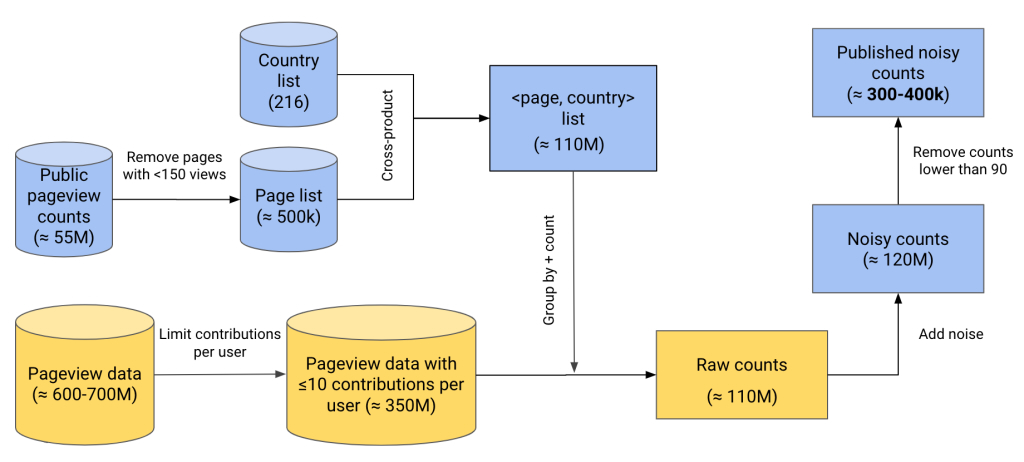
\includegraphics{images/wiki-pageview-differential-privacy-pipeline.jpg}

}

\caption{Triedman, Hal. ``Conceptual Steps of the Pageview Differential
Privacy Pipeline.'' Wikipedia, licensed under CC BY-SA 4.0.
https://diff.wikimedia.org/2023/06/21/new-dataset-uncovers-wikipedia-browsing-habits-while-protecting-users/screenshot-2023-05-23-at-10-34-18-am/.
License: https://creativecommons.org/licenses/by-sa/4.0/.}

\end{figure}%

\subsection{Methods}\label{methods}

For models built using this data to be effectively utilized by
decision-makers, they must accurately estimate the expected number of
cases. Since these values are influenced by the model specified and data
used, the methods used in this paper draws from prior work to determine
how to approach the task. When it comes to assessing the predictive
value of online search activity for disease incidence, there are two
primary types of methods: (1) lag analysis, which involves lagging
either cases or pageviews to detect leading indicators, and (2)
statistical forecasting methods, that range in complexity
(\citeproc{ref-generous2014}{Generous et al. 2014}).

While lag analysis has resulted in mixed findings
(\citeproc{ref-cervellin2017}{Cervellin, Comelli, and Lippi 2017};
\citeproc{ref-chrzanowski2021}{Chrzanowski et al. 2021};
\citeproc{ref-polgreen2008}{Polgreen et al. 2008};
\citeproc{ref-yang2011}{Yang et al. 2011}), both Du et al.~and Yan et
al.~apply this method to Google Trends Index data in the context of
mpox, finding that significant lag-correlation between GTI and daily
mpox cases with online search activity preceding cases, showing that the
approach may hold some promise (\citeproc{ref-du2023}{Du et al. 2023};
\citeproc{ref-yan2023}{Yan et al. 2023}). More advanced statistical
forecasting methods have also demonstrated impressive results
(\citeproc{ref-abbas2021}{Abbas et al. 2021};
\citeproc{ref-bernardo2013}{Bernardo et al. 2013};
\citeproc{ref-brownstein2009}{Brownstein, Freifeld, and Madoff 2009};
\citeproc{ref-hickmann2015}{Hickmann et al. 2015};
\citeproc{ref-sousa-pinto2020}{Sousa-Pinto et al. 2020}), however, they
often rely on large amounts of case data and high volumes of online
search activity over longer time periods, particularly when a seasonal
trend is present (e.g., COVID-19, influenza).

While statistical forecasting methods are powerful, epidemic parameters
are not always known during outbreaks of novel or understudied diseases.
As Generous et al.~argue, in such instances where epidemic parameters
are not well understood or a clear seasonal pattern cannot be
established, simpler methods may be more effective
(\citeproc{ref-generous2014}{Generous et al. 2014}). Building on
existing research, I test both approaches to evaluate their efficacy in
the context of the 2022-2024 mpox outbreak.

\section{Research Questions}\label{research-questions}

The primary question that this paper sets out to answer is whether
Wikipedia pageviews data can effectively function as a data source for
predicting disease incidence during the 2022-2024 mpox outbreak,
specifically in the context of the United States. The decision to focus
on the United States is driven by the fact that it has reported the most
cases of any country, comprising 33.7\% of global cases (32,063 /
95,227), with cases continuing to be reported as of early 2024
(\citeproc{ref-cdc2023}{CDC 2023}; \citeproc{ref-whoshiny}{WHO 2024}).
This lends itself to time series modeling which benefits where data is
available. Moreover, the length of the outbreak enables the initial
period to be used to train a predictive model and a subsequent period to
be used to test whether the model's predictive value retains accuracy
over time. The United States also generates the highest number of
Wikipedia pageviews (\citeproc{ref-wikimedi}{{``Wikimedia Traffic
Analysis Report - Page Views Per Wikipedia Language - Breakdown,''}
n.d.}). This high volume of Wikipedia traffic increases the likelihood
that mpox-related Wikipedia articles will consistently receive pageviews
above the required threshold imposed by the Wikimedia Foundation in
order to be eligible for inclusion in the anonymized country-level
dataset.~

Supporting this central question are several sub-questions that delve
into specifics. First, I identify which mpox-related articles on
Wikipedia are most closely aligned with fluctuations in mpox case
numbers, potentially acting as indicators of disease spread.
Additionally, the paper seeks to determine the optimal time lag between
observed pageviews and reported mpox cases, which could help in
predicting future outbreaks more accurately. Moreover, the research
examines the adequacy of the predictive model being used---how well it
fits data from the initial period and whether it can be effectively
applied to later periods. A critical aspect of this analysis involves
distinguishing the influence of actual disease cases on Wikipedia
pageviews from other potential drivers like media coverage or scientific
interest. Understanding these dynamics is crucial for improving the
model's predictive power and reliability.

\section{Data and Methods}\label{data-and-methods}

\subsection{Data Sources}\label{data-sources}

To investigate the predictive value of Wikipedia pageviews toward mpox
case incidence during the 2022-2024 outbreak in the United States, this
paper primarily relies on daily confirmed case data from the U.S. CDC
and daily U.S. Wikipedia pageviews for mpox-related articles.
Additionally, it incorporates data on media coverage from GNews and
scientific publications from PubMed to consider other significant
factors influencing online public attention
(\citeproc{ref-adawi2017}{Adawi et al. 2017}).

\subsubsection{Mpox case data}\label{mpox-case-data}

Data on daily number of mpox cases are obtained directly from the U.S.
CDC website (\citeproc{ref-cdc2023}{CDC 2023}). Case data are compiled
through a reporting chain that involves state public health officials
and healthcare providers identifying and reporting cases to the CDC,
where figures are then aggregated at the national level prior to public
release (\citeproc{ref-mcquiston2023}{McQuiston 2023}). As of March 5,
2024, mpox cases have been reported by all 50 states, the District of
Columbia, and Puerto Rico (\citeproc{ref-cdcmap}{CDC 2024}). Data is as
of March 5, 2024 and contains cases reported between 10 May 2022 to 27
February 2024.

\begin{figure}[H]

{\centering 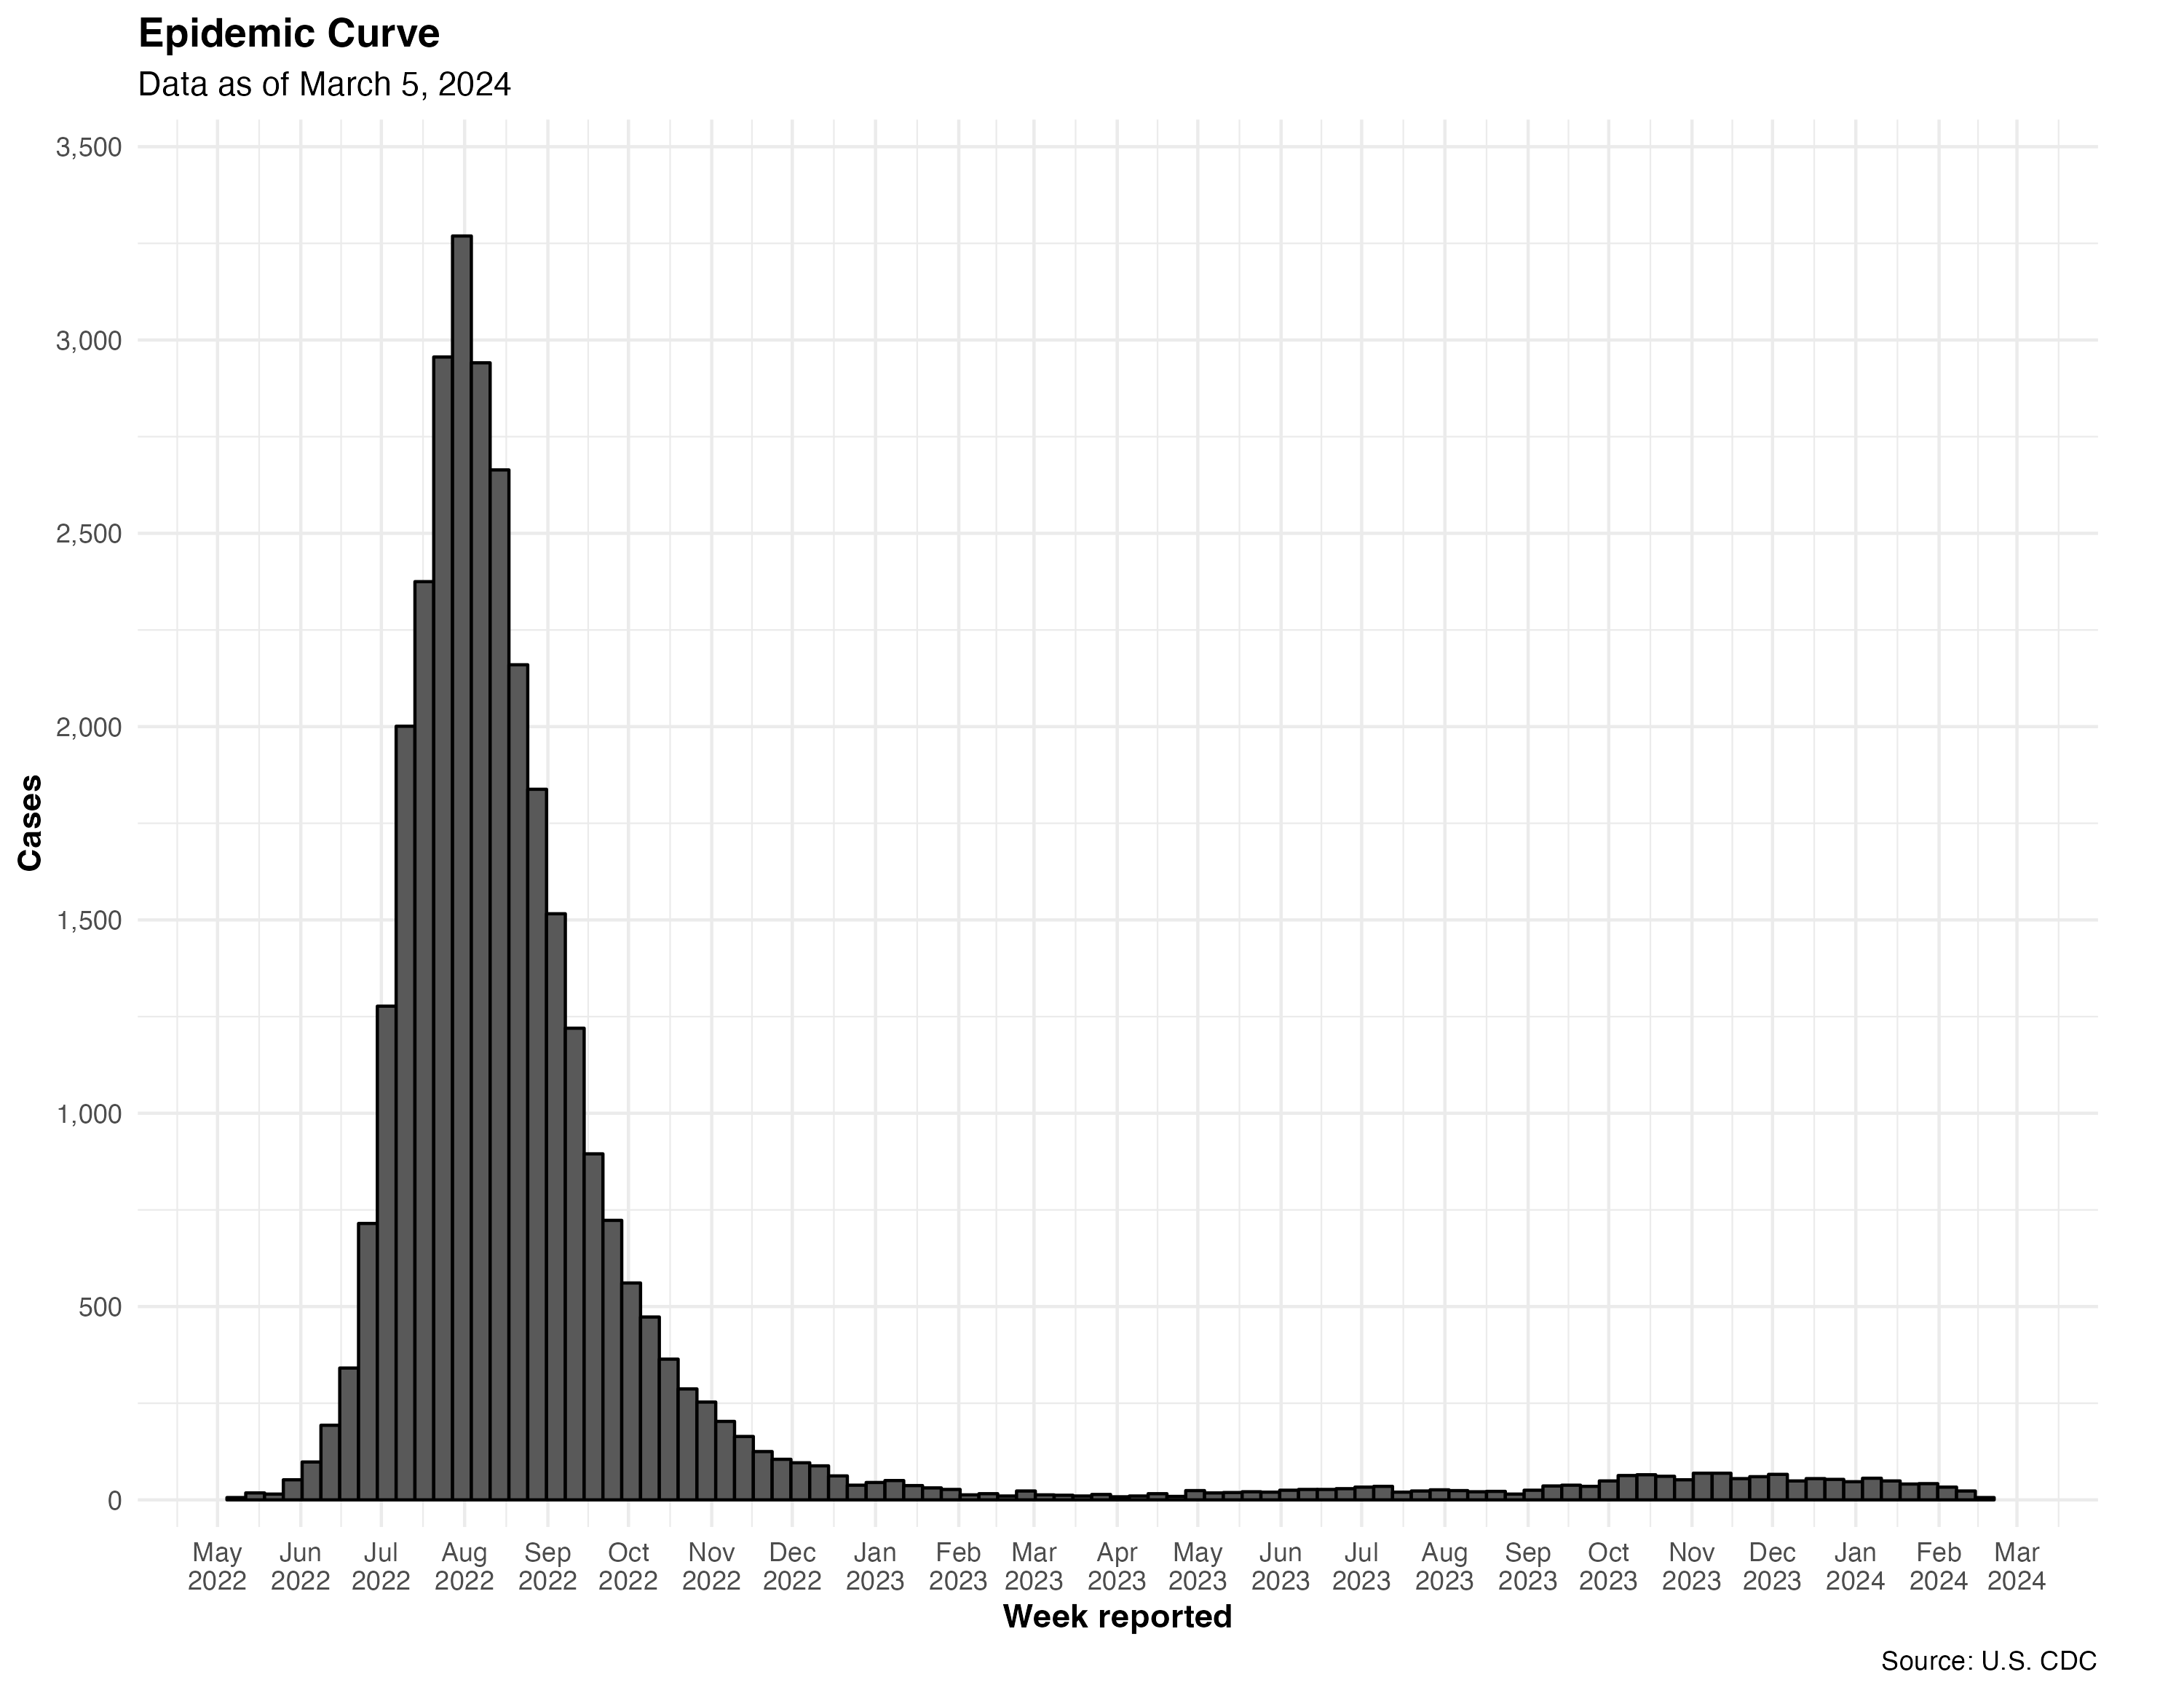
\includegraphics{images/cases.png}

}

\caption{Epidemic curve of U.S. mpox cases}

\end{figure}%

\subsubsection{Wikipedia pageview data}\label{wikipedia-pageview-data}

Daily anonymized statistics for mpox-related English-language Wikipedia
pageviews from the United States were sourced from the Wikimedia
Foundation. English-language articles are used since data on U.S.
pageviews for other Wikipedia language projects are limited. This
decision is not anticipated to substantially impact the analysis since
English-language Wikipedia accounts for approximately 90\% of the United
States' total pageviews.

\begin{figure}[H]

{\centering 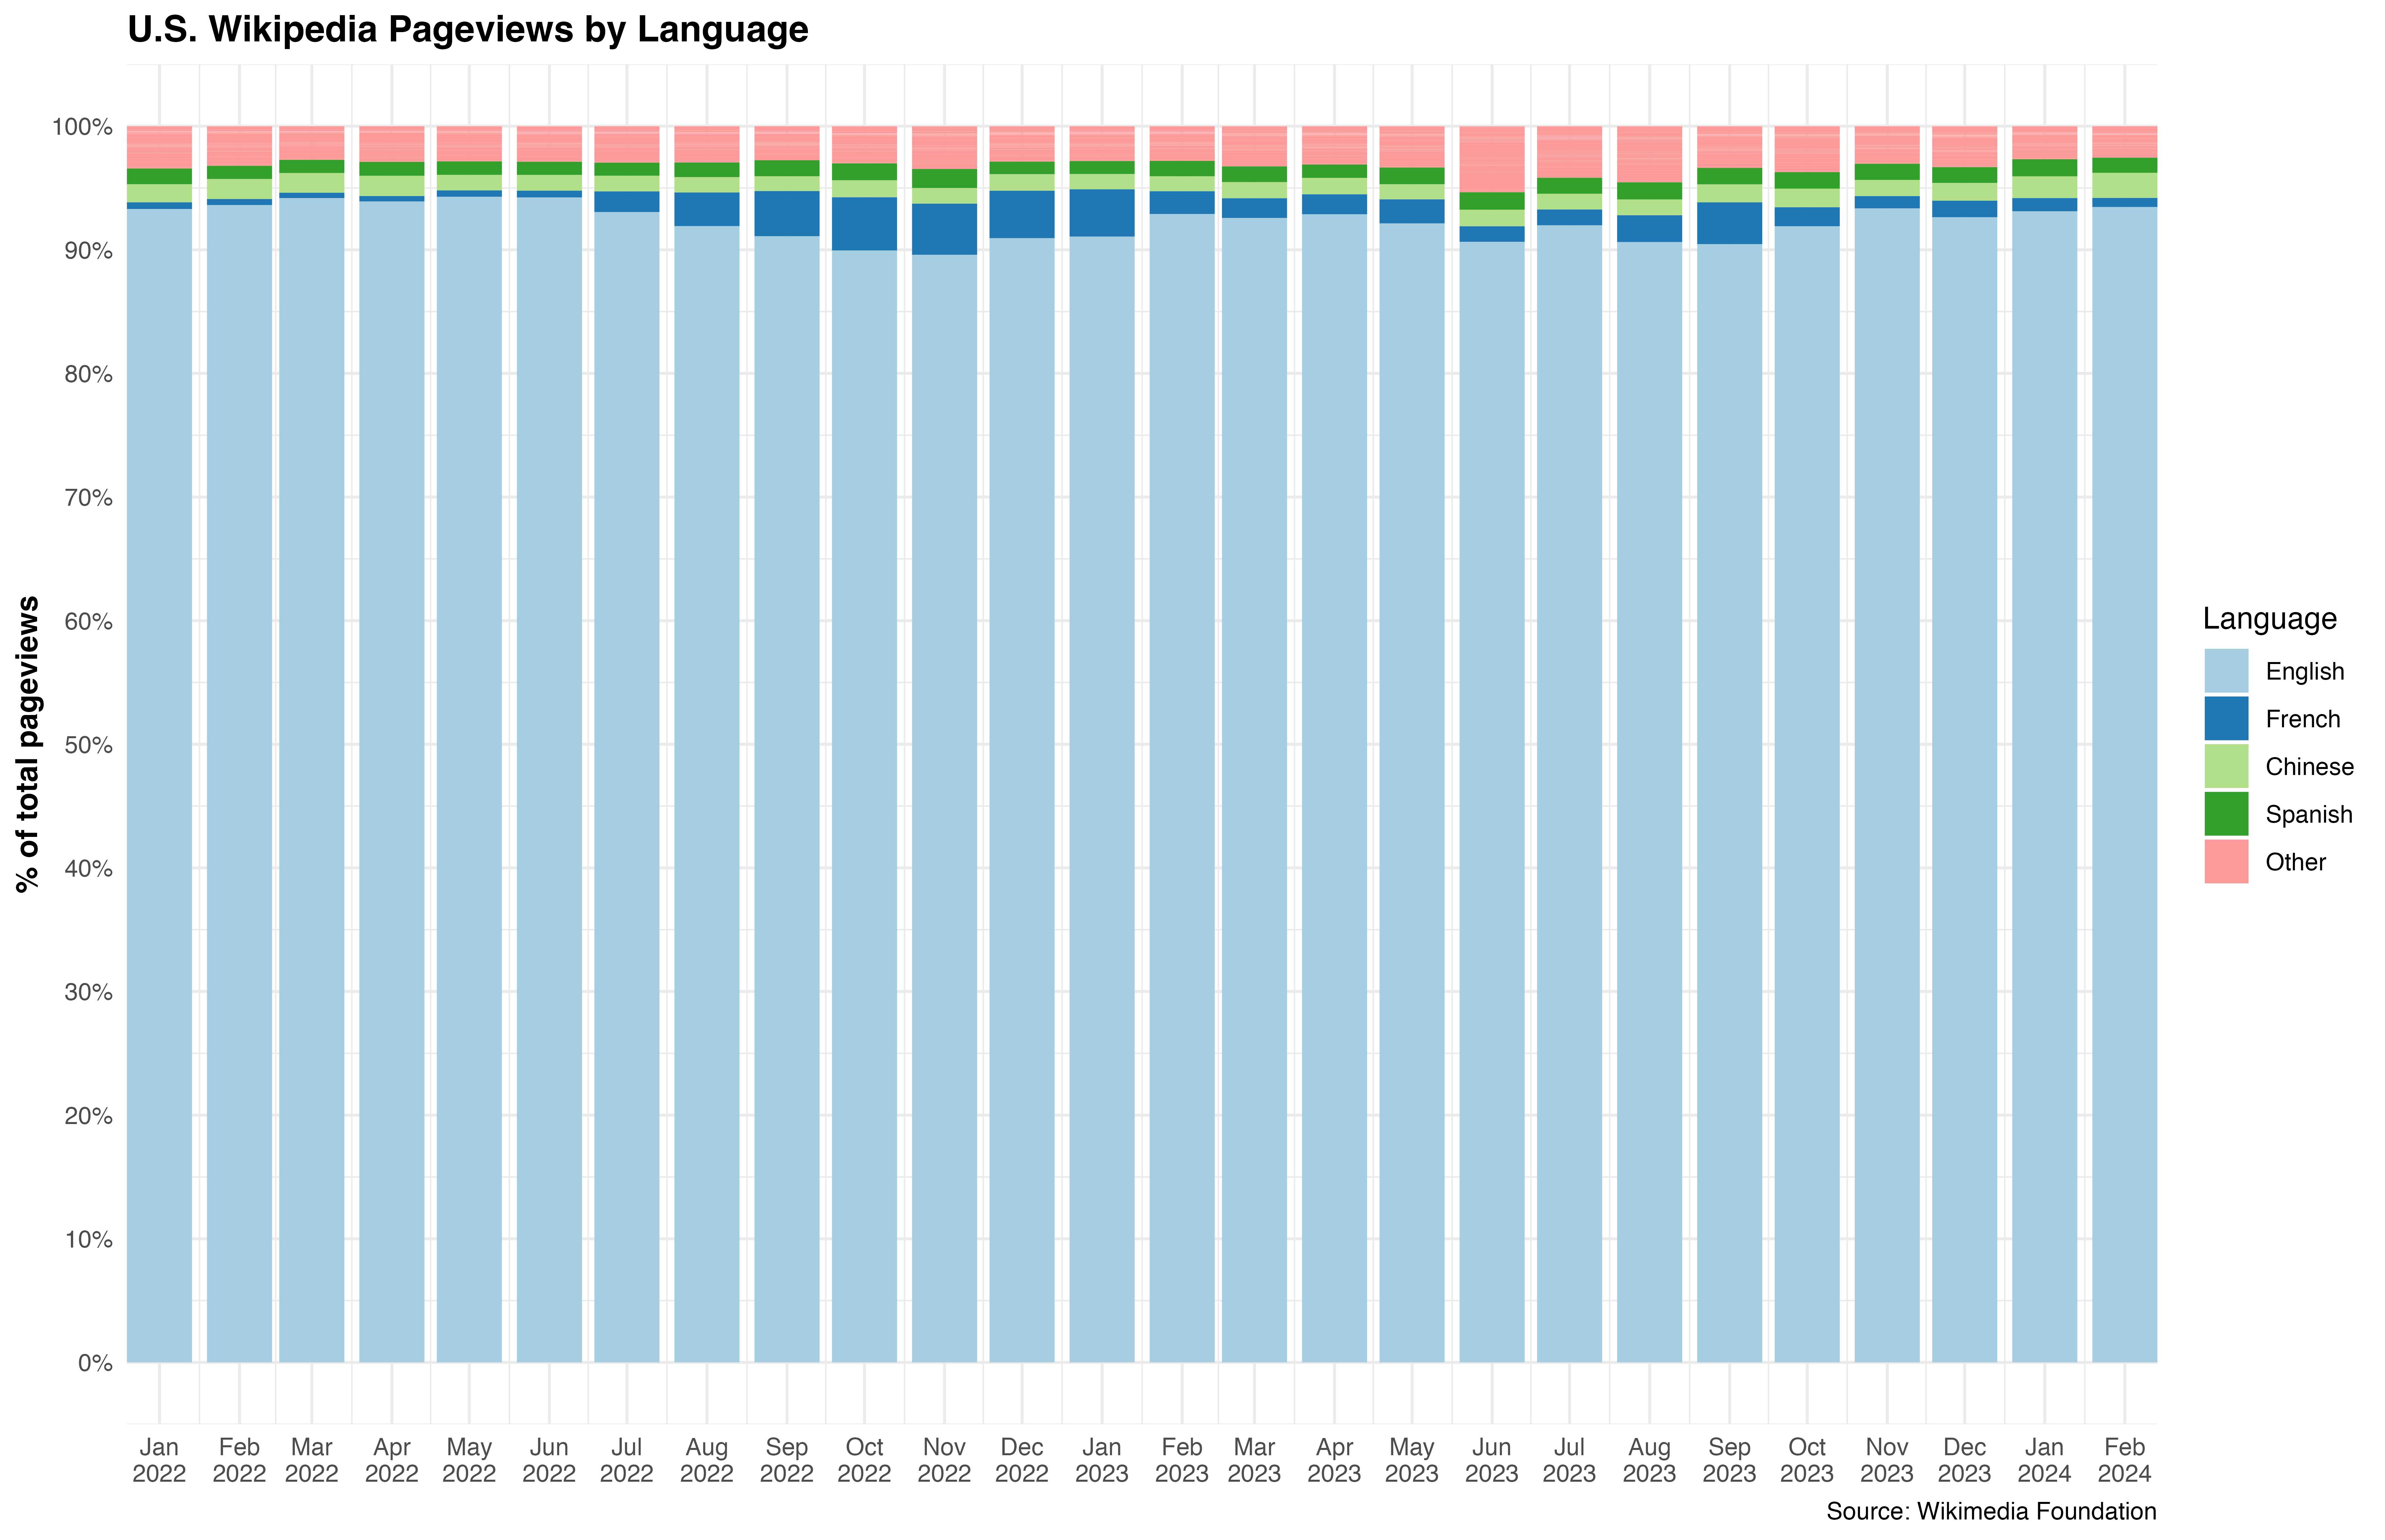
\includegraphics{images/wiki-project-views.png}

}

\caption{U.S. Wikipedia pageviews by language}

\end{figure}%

The data collection process involved identifying key Wikipedia articles
related to mpox, starting with ``Mpox'' and ``Monkeypox virus'' from the
English-language Wikipedia. Using the Wikimedia Analytics Query Service
(AQS) REST API via the \texttt{\{WikipediR\}} package
(\citeproc{ref-wikipedir}{Keyes, Tilber, and Schmid 2024}), a
comprehensive list of 451 linked articles was narrowed down through
manual review to 39 directly related to mpox, excluding those primarily
documenting the 2022-2024 outbreak. Additional articles on mpox symptoms
like ``Lesion'' and ``Myalgia'' were also included, informed by WHO
guidelines and symptomatology reports (\citeproc{ref-mpox_cif}{WHO
2023b}, \citeproc{ref-whoshiny}{2024}).

\begin{figure}[H]

{\centering 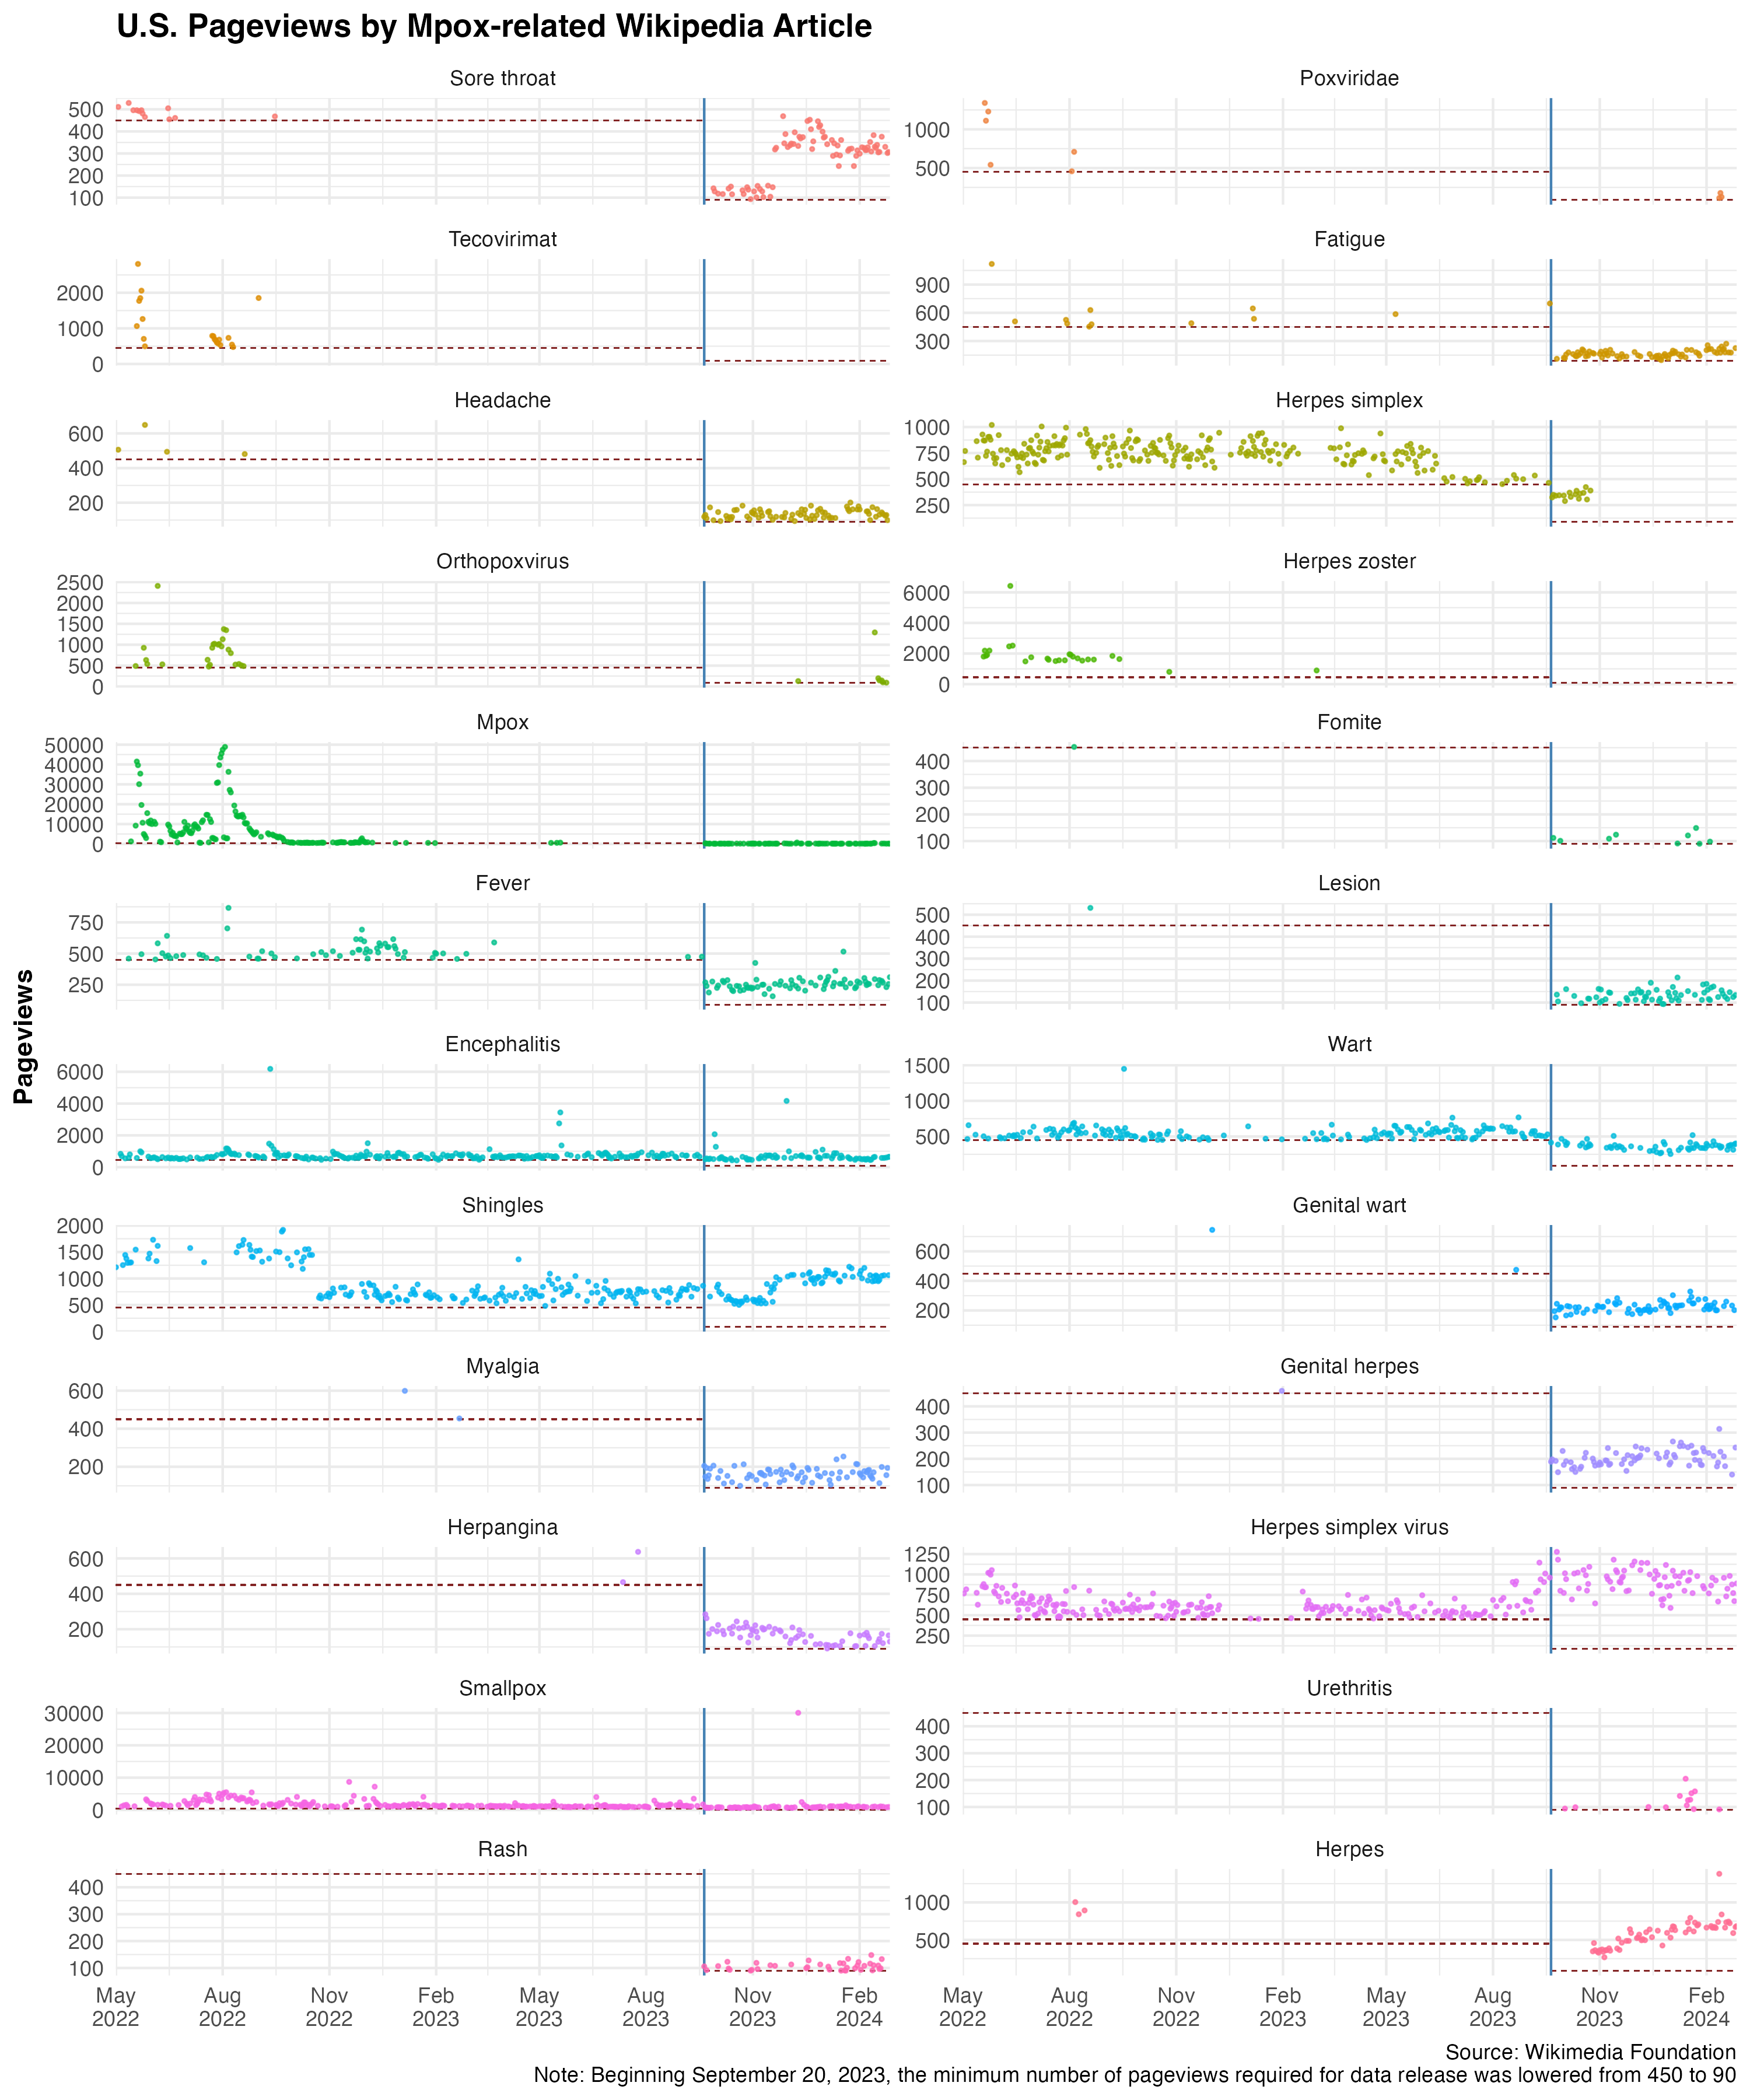
\includegraphics{images/pageviews-mpox-related.png}

}

\caption{U.S. pageviews by mpox-related Wikipedia article}

\end{figure}%

Daily anonymized pageview statistics for mpox-related Wikipedia articles
exceeding the Wikimedia Foundation's privacy threshold were obtained and
subsequently normalized by dividing daily views per article by total
monthly pageviews of English-language Wikipedia from the U.S. which were
accessed via the Wikimedia AQS REST API.

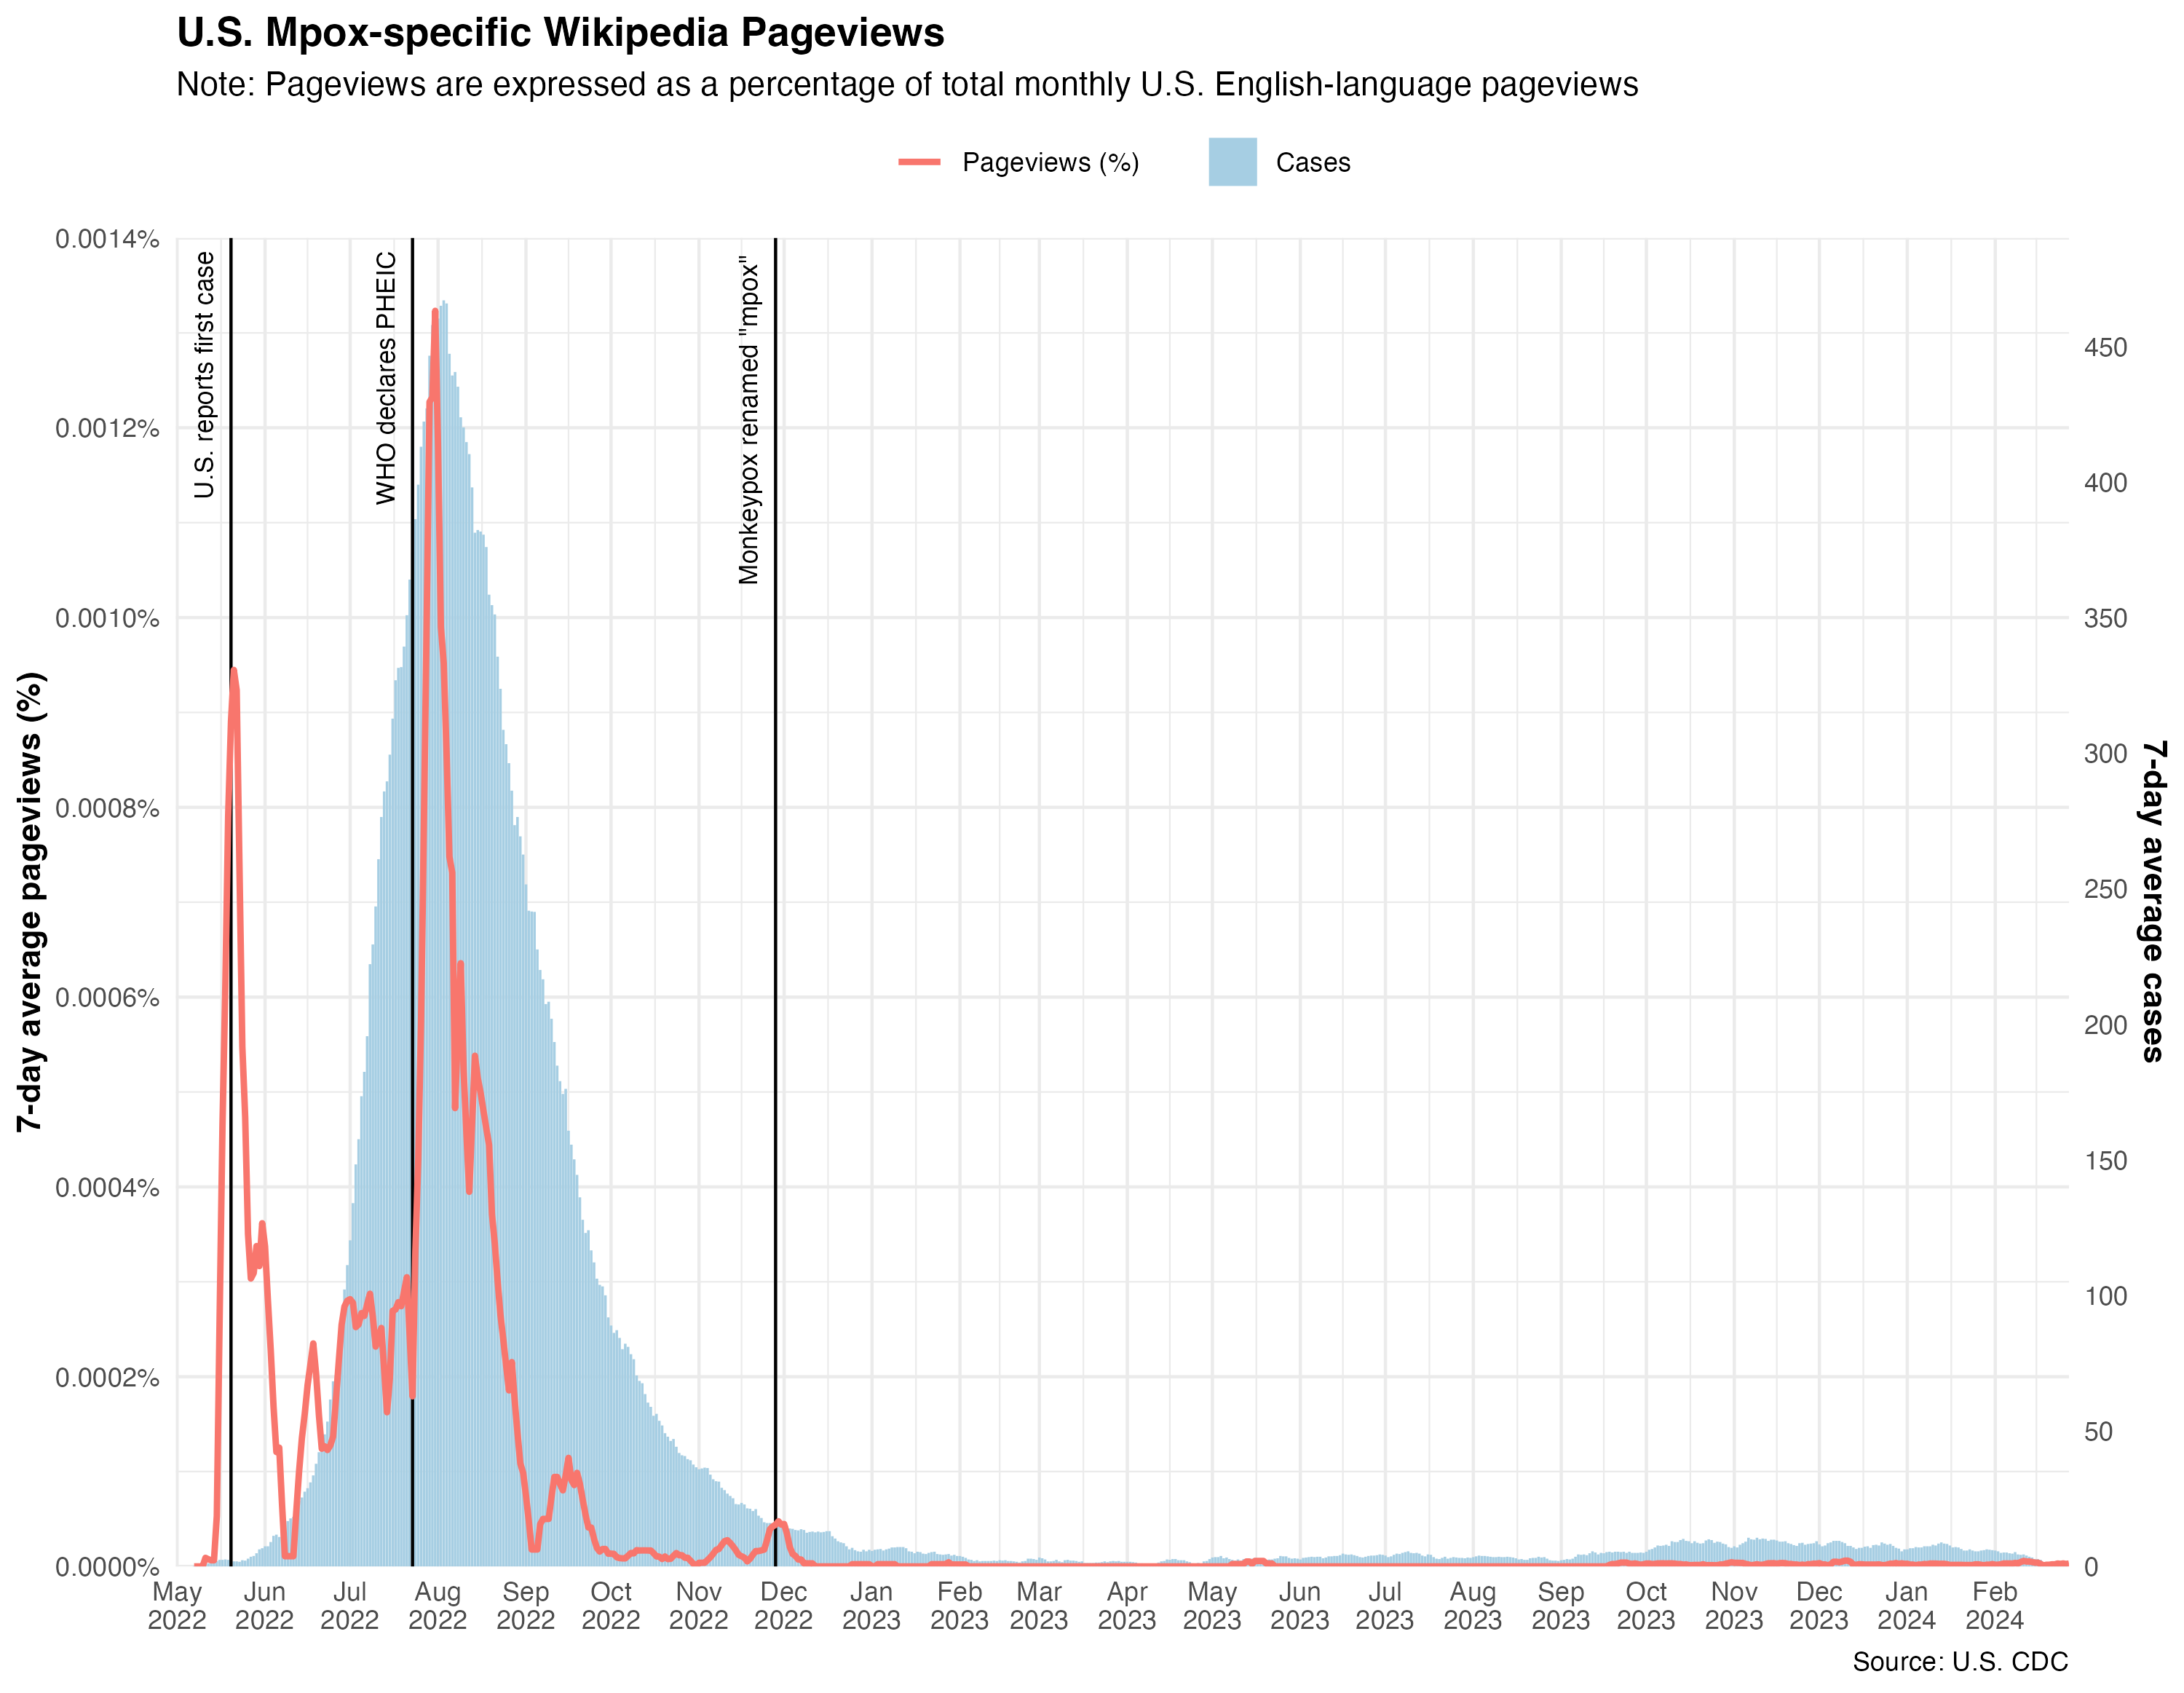
\includegraphics{images/cases-&-pageviews-rolling-avg.png}\\

\subsubsection{Media coverage data}\label{media-coverage-data}

In order to account for the impact of media coverage on public attention
toward mpox, data on the daily number of mpox-related articles published
during the study period are obtained from GNews API
(\citeproc{ref-gnewsap}{{``GNews API: Your Gateway to the Power of News
APIs''} 2024}). The GNews database contains tens of millions of articles
from over 60,000 sources (\citeproc{ref-gnewsap}{{``GNews API: Your
Gateway to the Power of News APIs''} 2024}). Articles including
``monkeypox'' in the title or description from May 1, 2022 to November
27, 2022 are counted. Following WHO's recommendation on November 28,
2022 that monkeypox be renamed to ``mpox,'' articles including either
``monkeypox'' or ``mpox'' in the title or description are then counted
toward the total. (\citeproc{ref-whoreco}{WHO 2022c}).

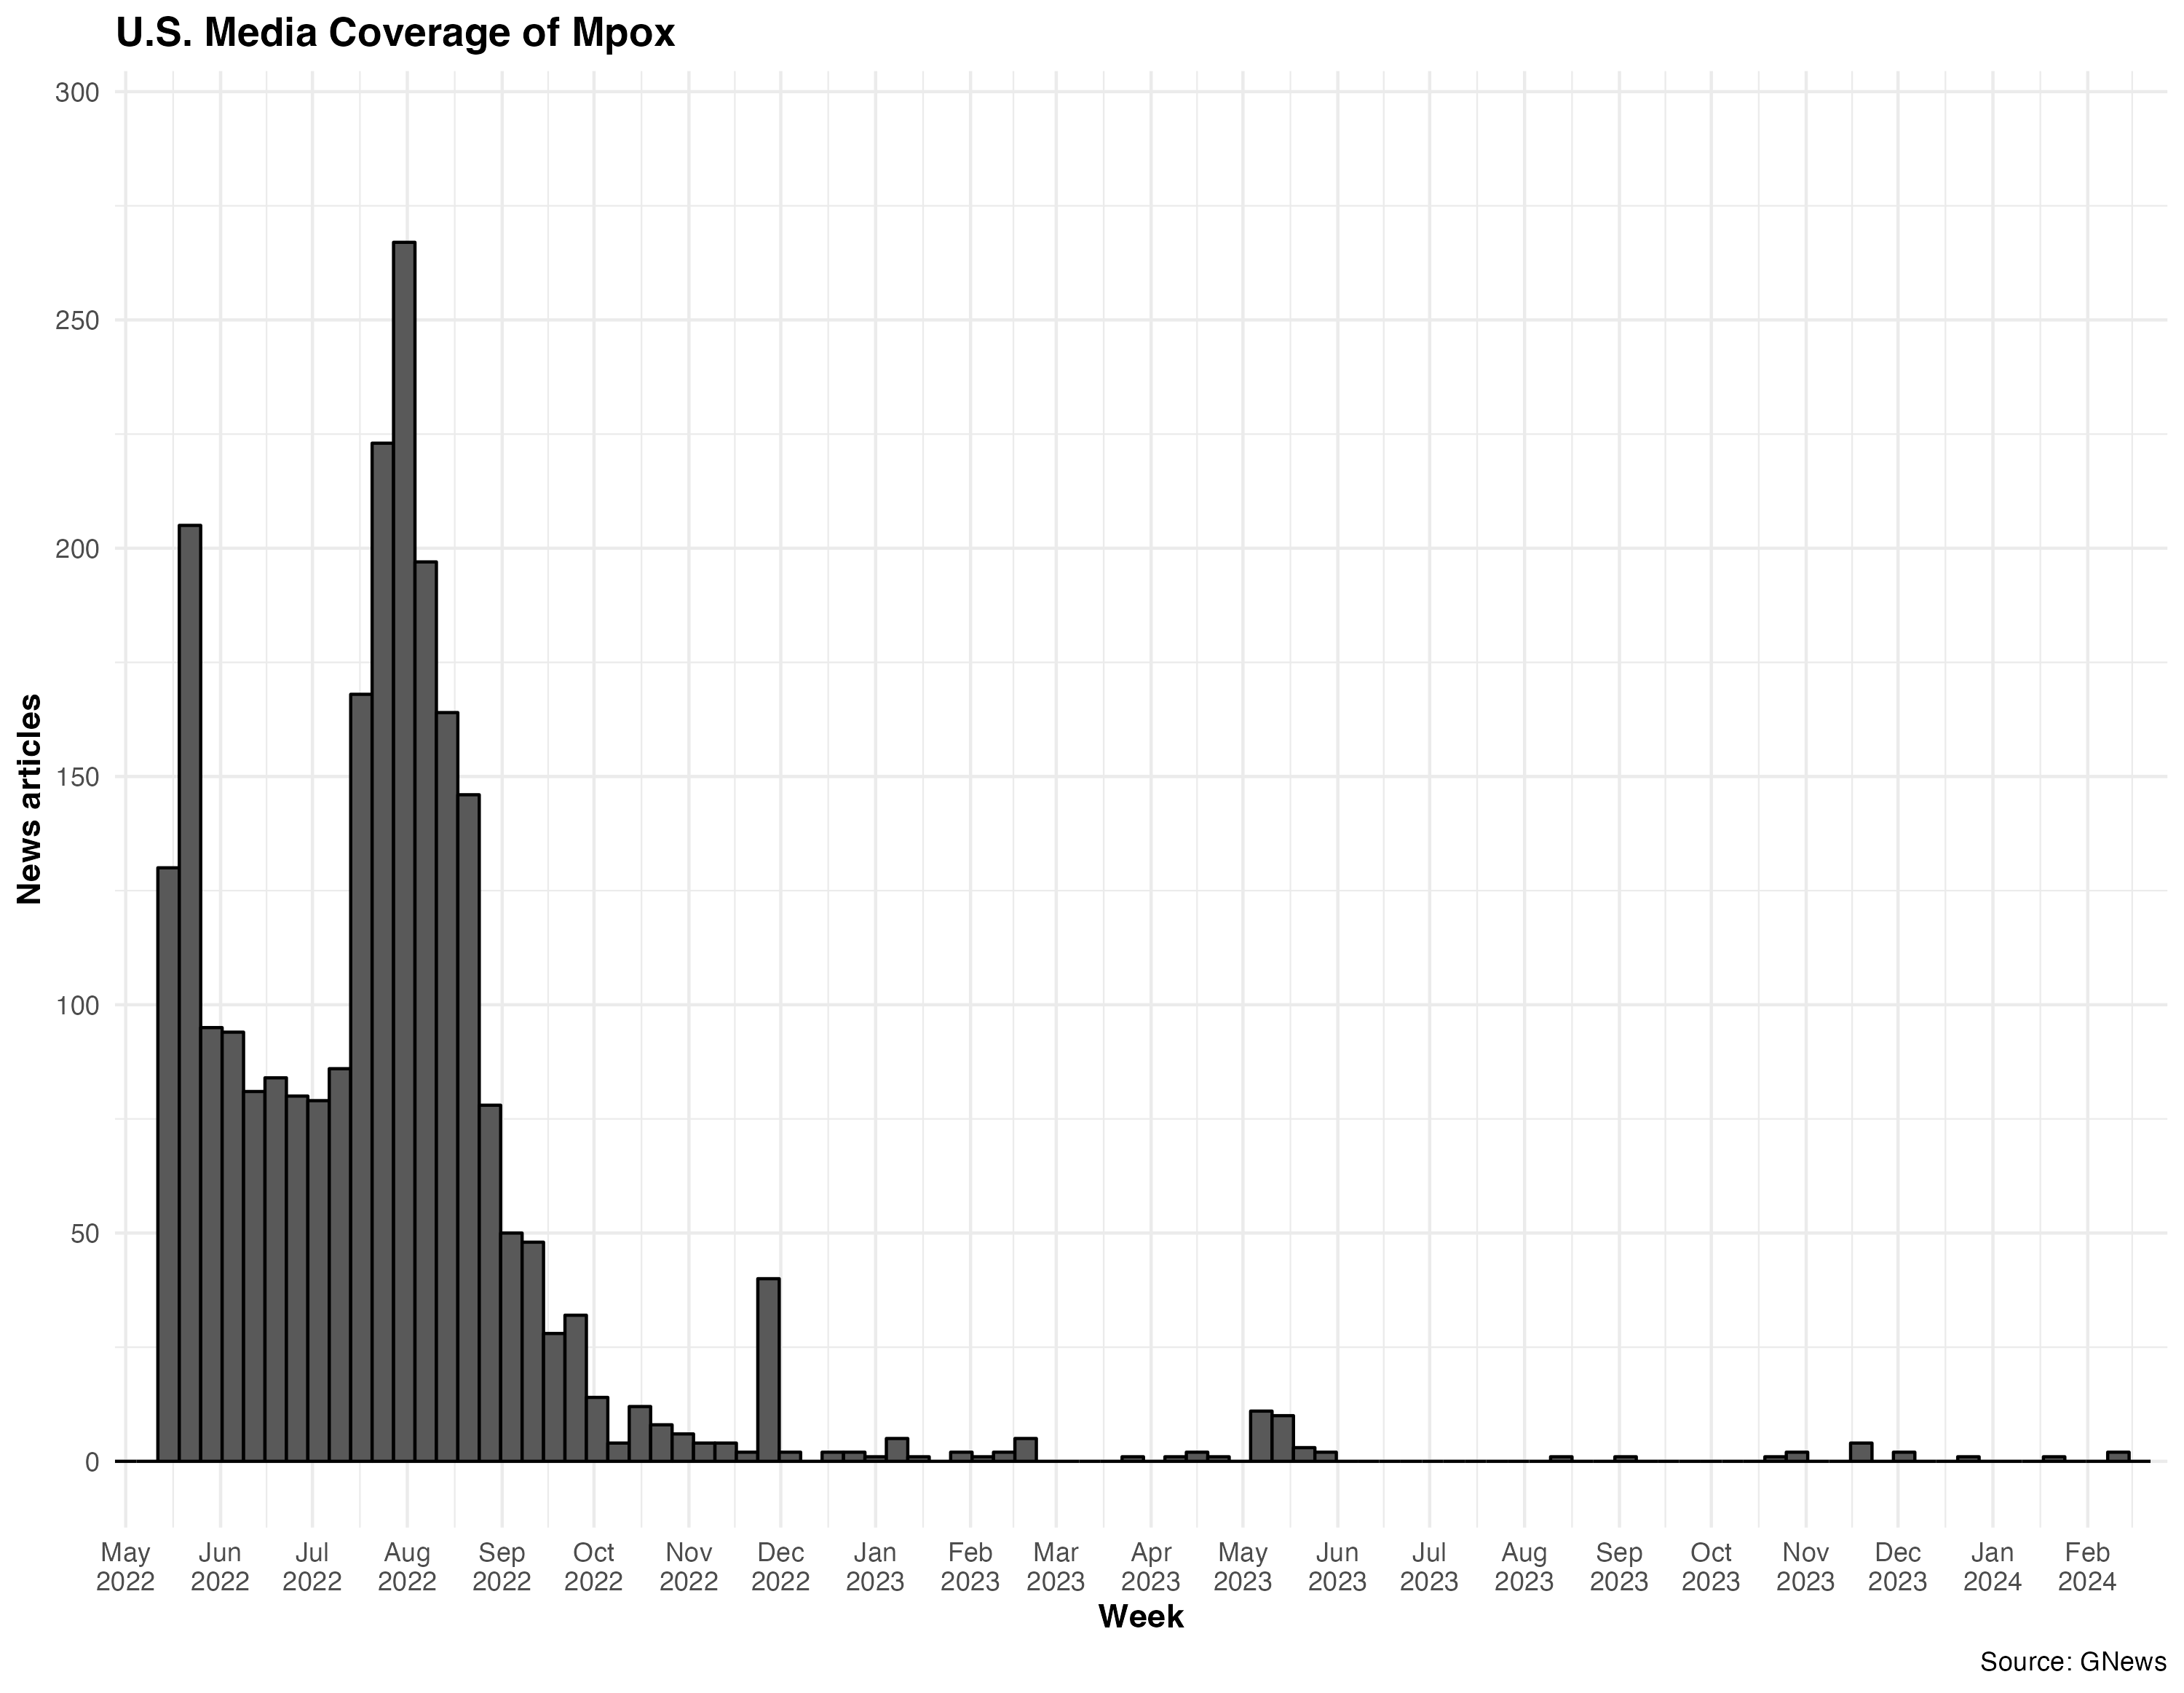
\includegraphics{images/mpox-news.png}\\

\subsubsection{Scientific interest data}\label{scientific-interest-data}

Data on scientific articles published from January 1, 2022, to February
27, 2024, related to mpox were retrieved from the PubMed database to
assess the impact of scientific interest on online attention towards the
disease. The \texttt{\{rentrez\}} package
(\citeproc{ref-winter2020}{Winter, Chamberlain, and Guangchun 2020}) was
used to extract papers from PubMed that mentioned ``monkeypox'' or
``mpox'' in their titles, descriptions, or Medical Subject Headings
(MeSH), with duplicates and missing titles removed to maintain data
integrity. Where specific publication dates were missing, e-publication
dates were used, with a note that aggregating data on a weekly basis
reduces any resulting bias in daily publication counts.

\begin{figure}[H]

{\centering 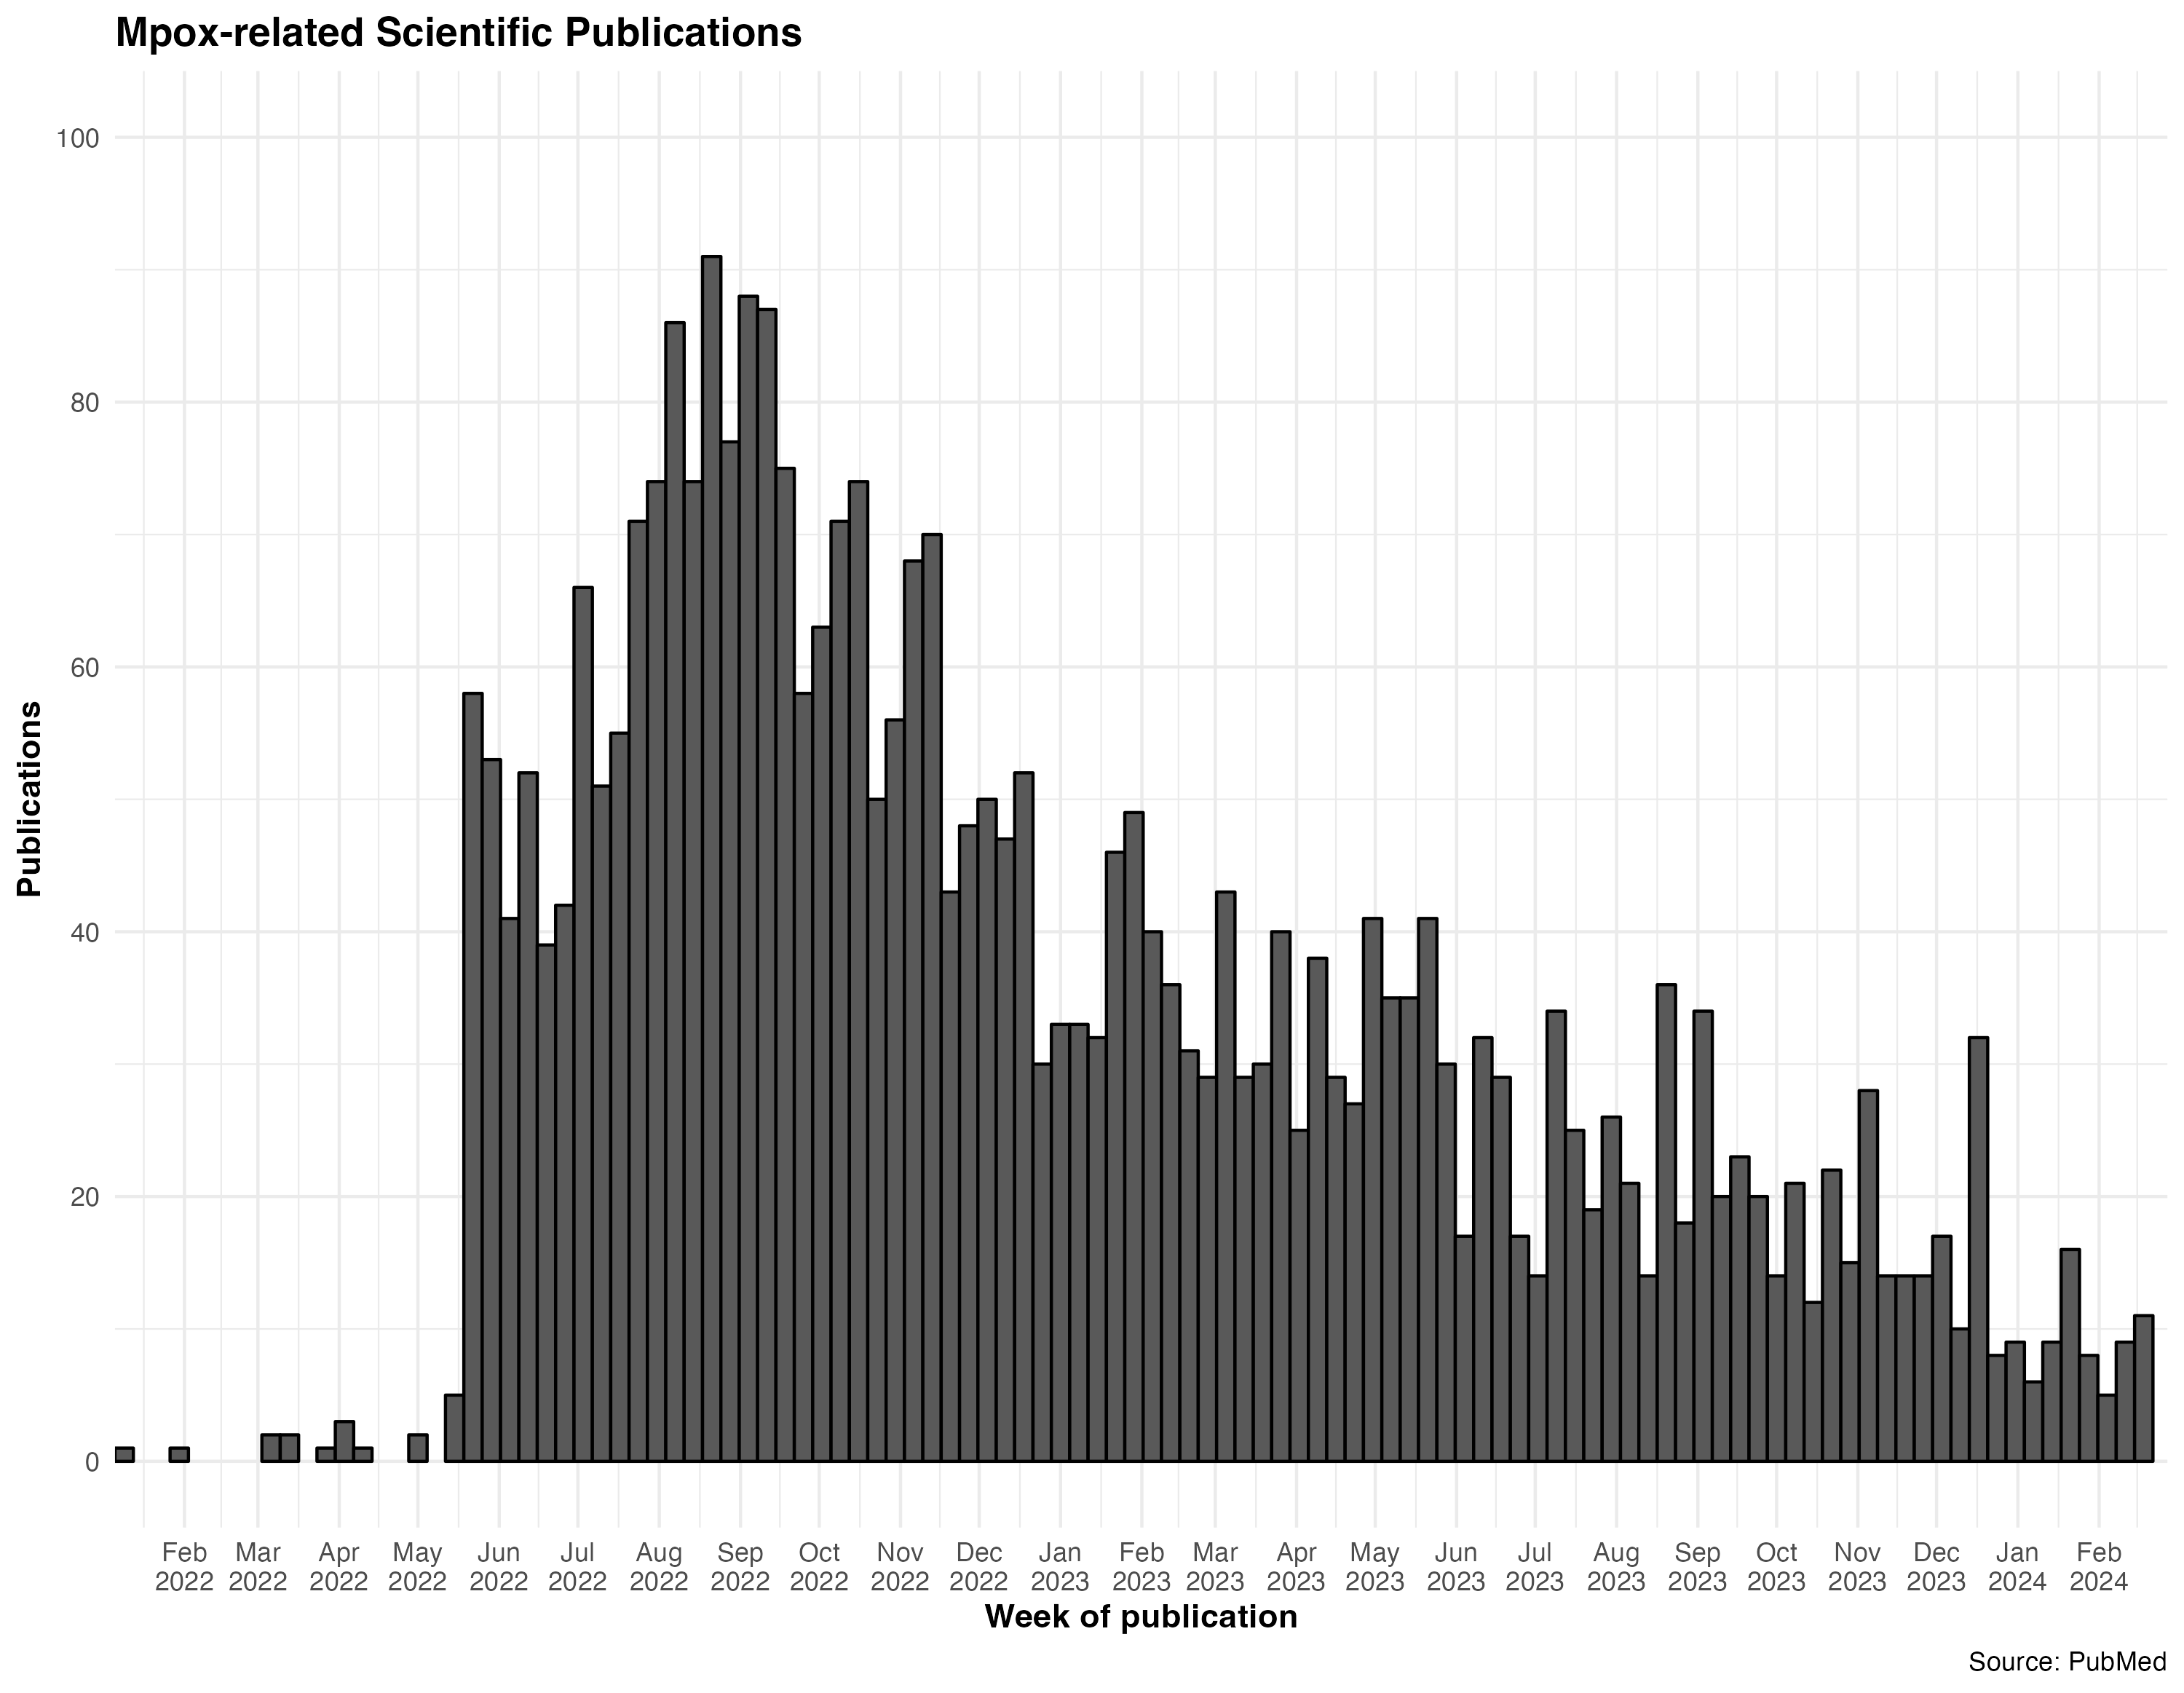
\includegraphics{images/mpox-studies.png}

}

\caption{Mpox-related scientific publications}

\end{figure}%

\subsection{Methods}\label{methods-1}

My proposed approach involves implementing several quantitative methods.
First, I perform a lag analysis, taking inspiration from the work of Yan
et al.~and Du et al~ (\citeproc{ref-yan2023}{Yan et al. 2023};
\citeproc{ref-du2023}{Du et al. 2023}). Next, I construct a multivariate
regression model and test its ability to accurately predict mpox cases,
drawing inspiration from various sources (\citeproc{ref-adawi2017}{Adawi
et al. 2017}; \citeproc{ref-generous2014}{Generous et al. 2014}).
Finally, I perform impulse response and Granger-causality tests to
assess the directionality of the relationship between the mpox cases and
pageviews (\citeproc{ref-yan2023}{Yan et al. 2023}). All analysis is
performed using R version 4.3.3 (\citeproc{ref-rformac}{Statistical
Computing 2024}).

\subsubsection{Lag analysis}\label{lag-analysis}

In the first stage of the analysis, a lag analysis was conducted to
investigate the relationship between mpox incidence and online public
attention as indicated by Wikipedia pageviews, using 7-day rolling
averages of both mpox cases and normalized pageviews to smooth the data.
To capture both immediate and delayed reactions, the 7-day rolling
averages of mpox cases were iteratively lagged from -35 to 35 days,
where a positive lag indicates future cases relative to pageviews, and a
negative lag looks at past cases. Spearman correlation coefficients were
used to measure the strength and direction of association due to the
data's non-normal distribution (\citeproc{ref-schober2020}{Schober and
Vetter 2020}). This analysis was carried out individually for each
mpox-related article within the dataset to identify patterns specific to
different content types. The entire study period from May 10, 2022, to
February 27, 2024, was analyzed, matching the availability of mpox case
data.

\subsubsection{Predictive model}\label{predictive-model}

In the next stage, I model the relationship between Wikipedia pageviews
and the incidence of mpox using multivariate linear regression to assess
how well simple models can fit to mpox case numbers. Four distinct
models were formulated using the 7-day rolling average of mpox cases as
the dependent variable and different configurations of independent
variables. The first model is based only on a 7-day rolling average of
cumulative normalized pageviews for ``Mpox'' and ``Monkeypox virus''
articles.~

\[
cases_t = \beta_0 + \beta_1 \times pageviews_{mpox, t}+ \epsilon_t
\]

Taking inspiration from Generous et al., the second model incorporates
the 7-day rolling averages of normalized pageviews for mpox-related
articles that were estimated to have an absolute Spearman correlation
greater than 0.5 based on the lag analysis
(\citeproc{ref-generous2014}{Generous et al. 2014}).~

\[
cases_t = \beta_0 + \sum \beta_i \times pageviews_{i, t}+ \epsilon_t
\]

The third model combines the 7-day rolling average of cumulative
normalized pageviews for ``Mpox'' and ``Monkeypox virus'' articles with
key covariates, namely the 7-day rolling averages for news articles and
scientific publications that mention ``mpox'' or ``monkeypox.''~

\hfill\break
\[
cases_t = \beta_0 + \beta_1 \times media_t + \beta_2 \times academia_t + \beta_3 \times   pageviews_{mpox, t}+ \epsilon_t
\]\\

The final model uses pageviews from the included mpox-related articles
along with the same covariates for media coverage and scientific
interest.

\[
cases_t = \beta_0 + \beta_1 \times media_t + \beta_2 \times academia_t + \sum \beta_i \times pageviews_{i, t}+ \epsilon_t
\]\\

The models were then fit to data from May 10, 2022 to September 19,
2023. This period ranges from the date of the United States' first
reported mpox case to the date on which the Wikimedia Foundation altered
its approach to publicly releasing pageview statistics. Using the fit
models, predictions are generated for the period from September 20, 2023
to February 27, 2024 to assess the accuracy of these simple models when
applied to future data. To address missing values pageviews series,
values were imputed to be 449 for the initial period and 89 for the
later period. These values are just below the minimum pageview threshold
corresponding with their respective periods.

\subsubsection{Granger causality}\label{granger-causality}

In the final stage of the analysis, the strength and directionality of
the relationship between mpox cases and pageviews is explored using
impulse response and Granger-causality tests. The 7-day rolling average
of mpox cases and the 7-day rolling average of cumulative normalized
pageviews of the ``Mpox'' and ``Monkeypox virus'' Wikipedia articles are
used. The focus on these two articles is due to their specific relevance
to mpox and the relative completeness of their pageview data throughout
the study period. However, some data gaps exist due to internal
Wikipedia database issues or because some pageviews fell below the
minimum public release threshold. To address this and maintain the
continuity required for time series analysis, missing values were
imputed with a value of 449, which is just below the minimum inclusion
threshold for publication. While this approach slightly obscures trends
below this threshold, it ensures that the overall analysis remains
robust and unaffected by these minimal data losses.

A key assumption of this analysis is the stationarity of the time
series, which is verified using the Augmented Dickey-Fuller (ADF) test.
If a series is found to be non-stationary, it is first-order
differenced, a common technique that involves subtracting the previous
observation from the current one, before the ADF test is re-applied.
This differencing process may be repeated up to three times or until
both series achieve stationarity. Upon confirming stationarity, the data
is modeled using Vector autoregression (VAR), which captures the
temporal dynamics and potential feedback mechanisms between mpox-related
Wikipedia pageviews and mpox cases.

The interdependencies captured by the VAR model are further analyzed
using an impulse response function (IRF), projected over a 10-day
horizon with bootstrapping to establish confidence intervals. This
analysis helps with understanding the impact of a one-time shock in one
variable on the other over time. Additionally, Granger-causality tests
are conducted to determine if changes in one series can predict changes
in the other, and to check for any instantaneous causality between the
series. These steps help assess the dynamic interplay and predictive
power of mpox-related Wikipedia pageviews and mpox cases. This analysis
was performed using the entire study period from May 10, 2022 to
February 05, 2023, which corresponds with the time period for which the
pageviews data is largely complete in order to limit the amount of
imputation required to perform the time series analysis.

\section{Results}\label{results}

\subsection{Lag Analysis}\label{lag-analysis-1}

Of the 39 articles initially identified as relevant to mpox, only 14
contained enough data to be included in the lag analysis. For this
analysis, a minimum of 71 days of pageview data was required, matching
the 71 time lags used for calculating Spearman correlation. The lag
analysis distinguished between negative lags, suggesting mpox cases
influenced subsequent pageviews, and positive lags, indicating that
pageviews may have predicted later mpox cases.

Most articles, except for the one on Fever, demonstrated significant
correlations with mpox cases at various time lags, with five articles
(Encephalitis, Herpes simplex, Mpox, Smallpox, and Wart) maintaining a
positive correlation across all lag periods, and three articles (Genital
wart, Herpes simplex virus, and Sore throat) showing a consistent
negative correlation. Interestingly, some articles exhibited changes in
the direction of their correlation depending on the lag. For example,
the article on Fatigue displayed a positive correlation when mpox cases
preceded pageviews (negative lags) and a negative correlation for the
opposite scenario (positive lags), suggesting that mpox cases typically
lead to increased searches for fatigue, but not vice versa. Conversely,
the Genital herpes article suggested that an increase in pageviews could
potentially predict subsequent mpox cases.~

\begin{figure}[H]

{\centering 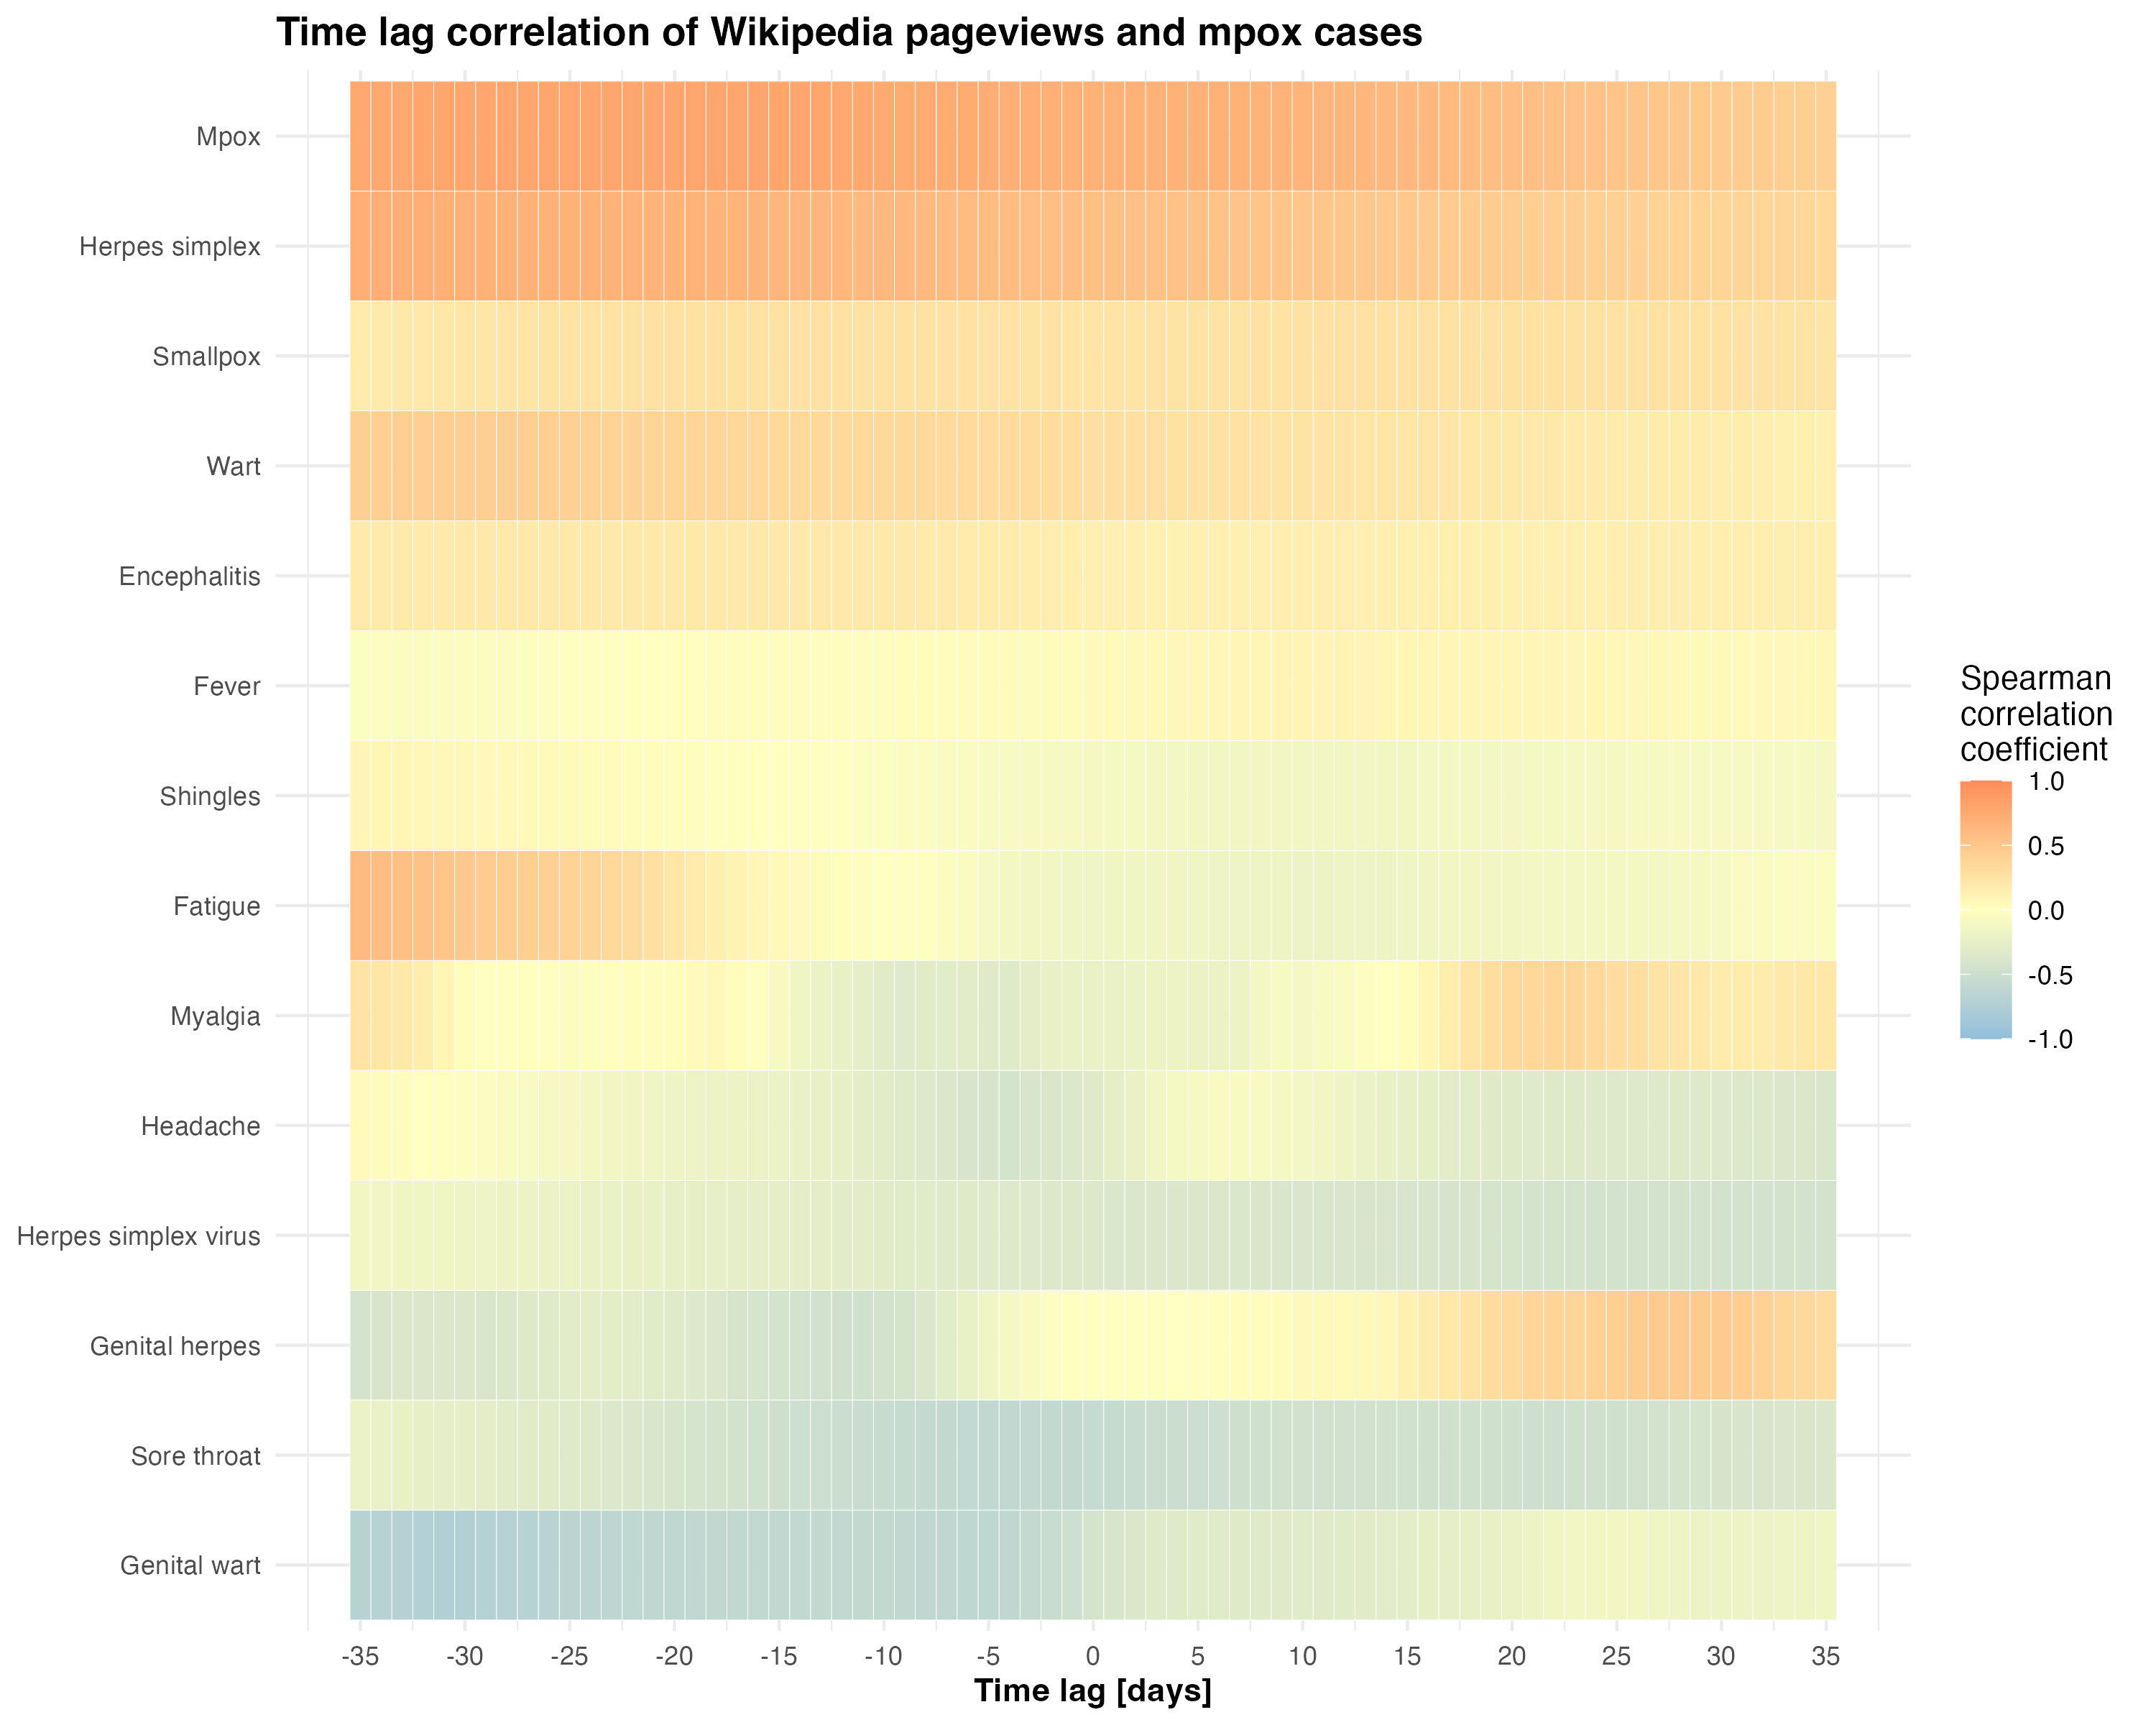
\includegraphics{images/spearman-correlation-heatmap.png}

}

\caption{Time lag correlation of Wikipedia pageviews and mpox cases}

\end{figure}%%
\begin{figure}[H]

{\centering 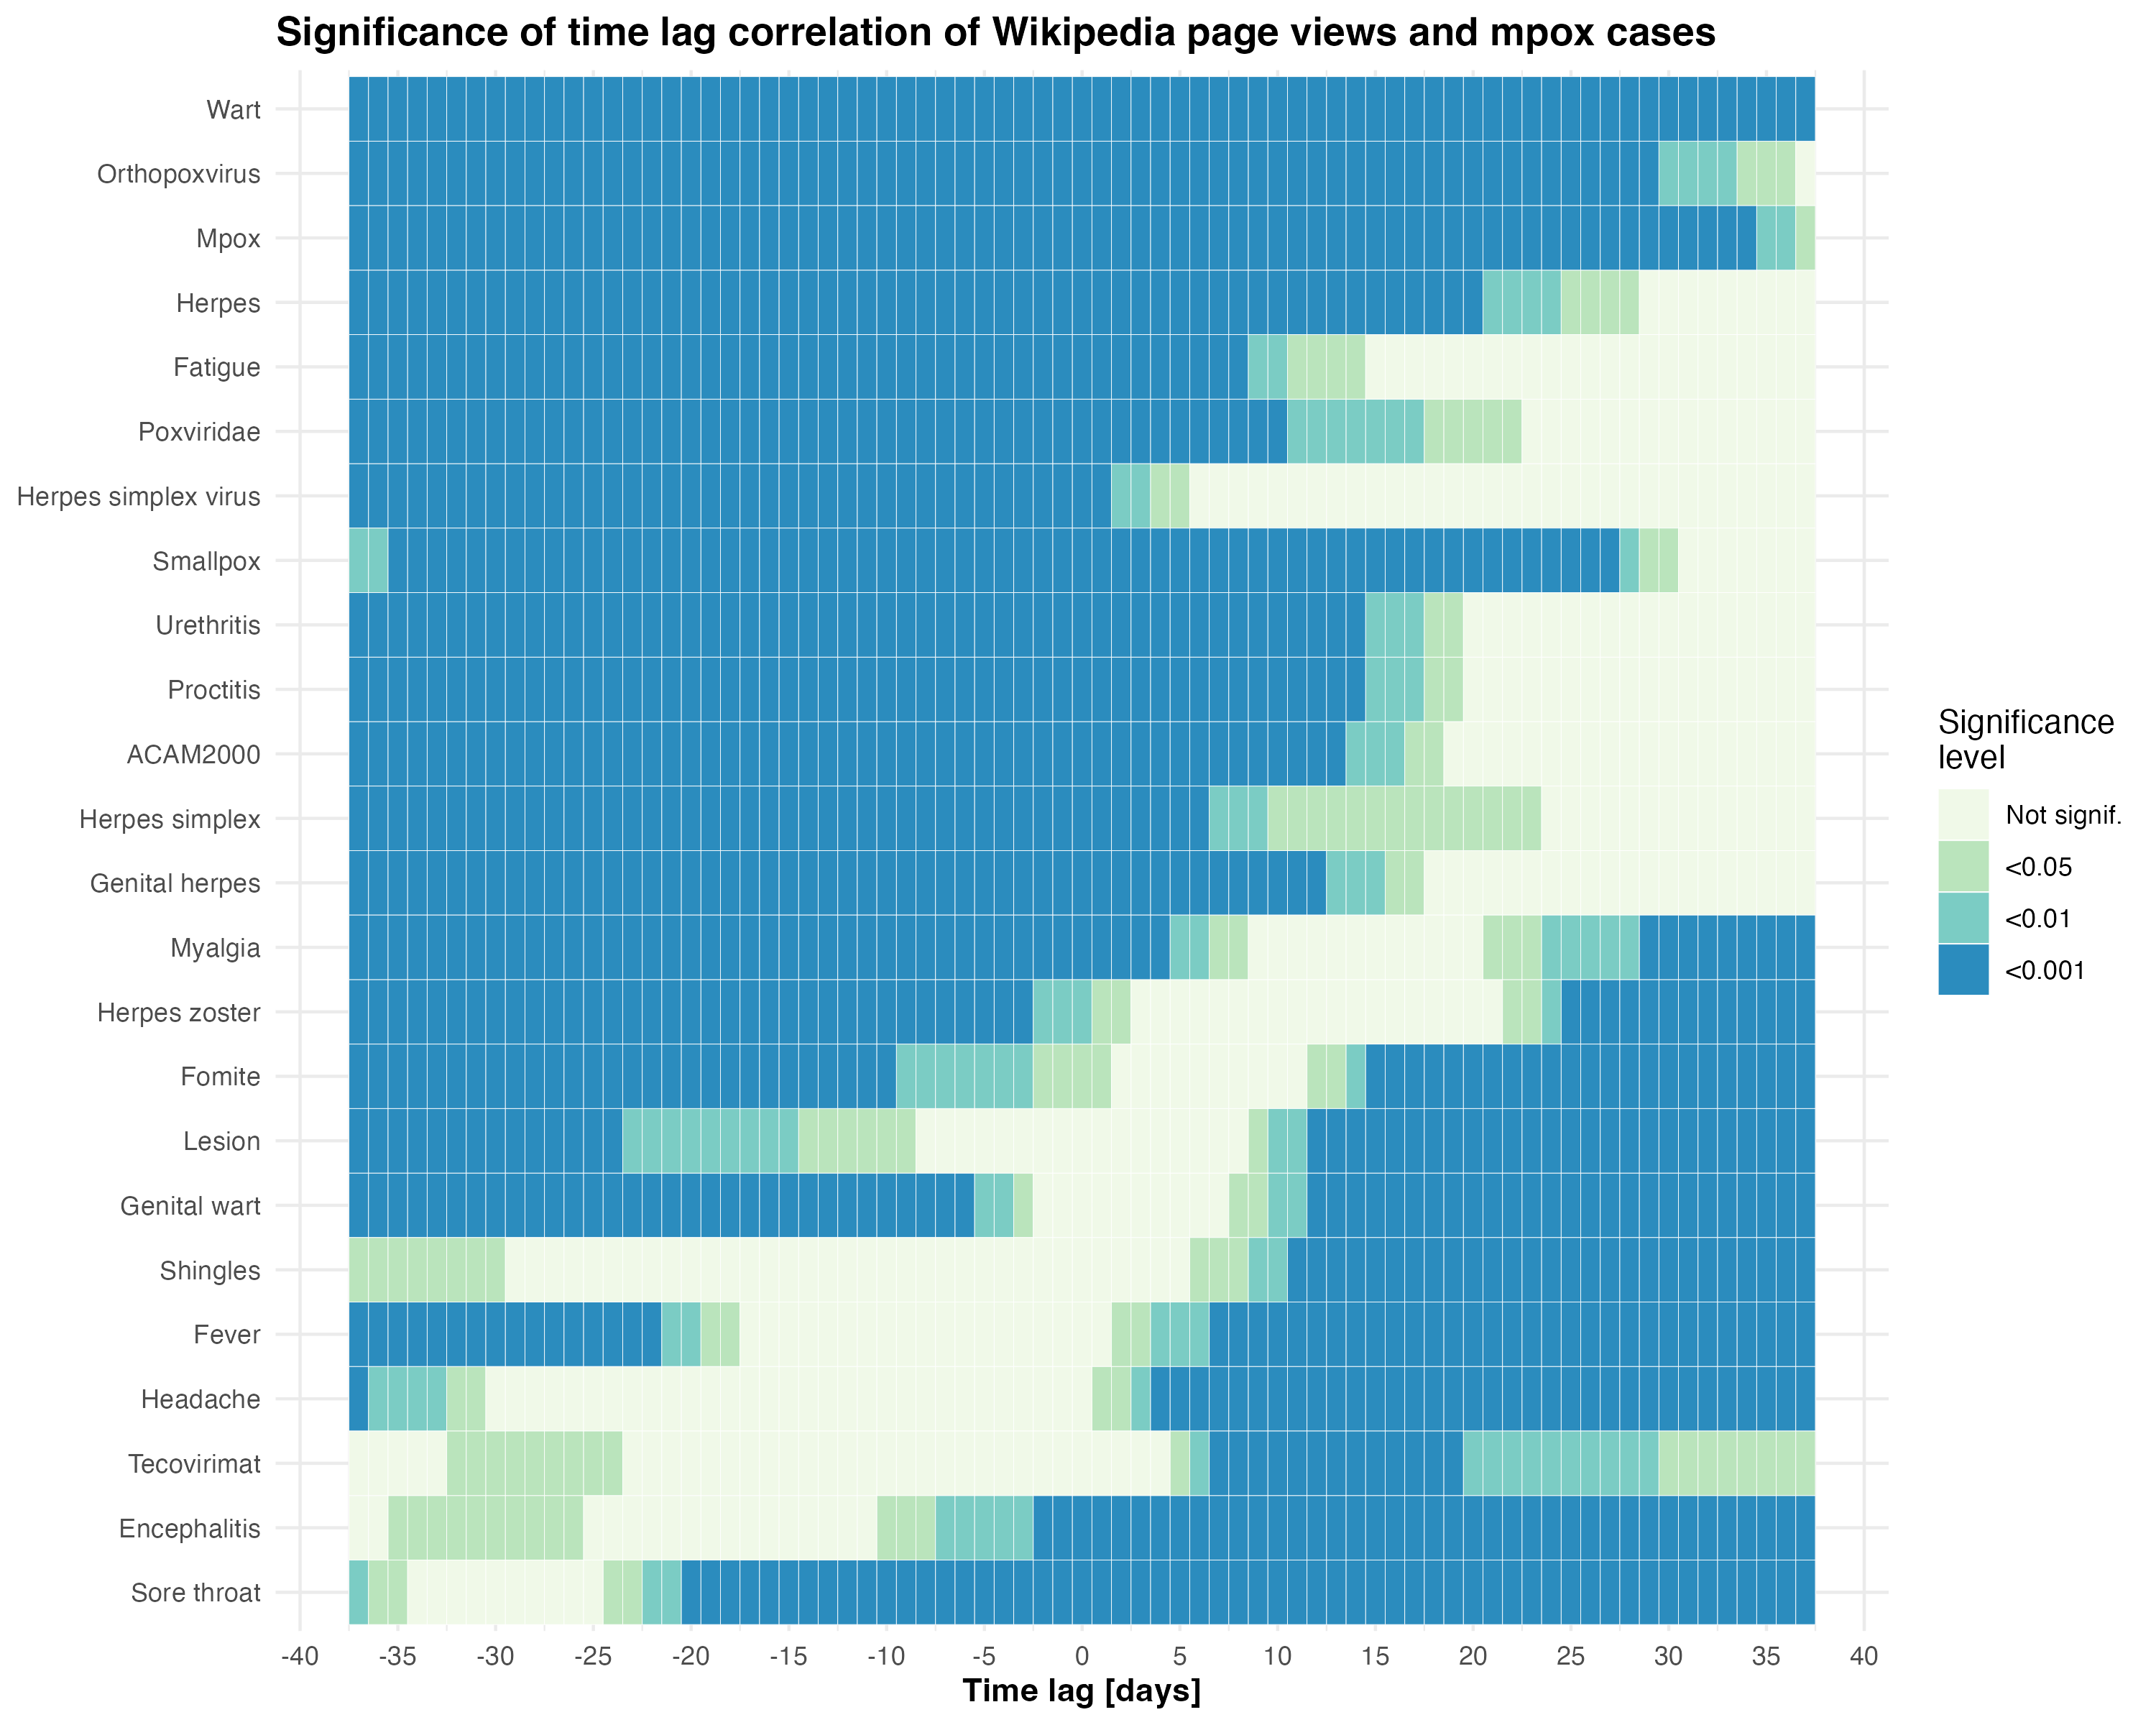
\includegraphics{images/spearman-pvalues-heatmap.png}

}

\caption{Significance of time lag correlation of Wikipedia pageviews and
mpox cases}

\end{figure}%

Articles with substantial correlation with mpox cases were selected for
inclusion in the next stage of the analysis. Only articles with a
Spearman correlation coefficient with an absolute value greater than 0.5
and at least 7 lag periods in which they were significantly correlated
with mpox cases were included. Statistical significance is defined as
\texttt{p} \textless{} 0.05. As a result, the following articles were
selected: Fatigue, Genital wart, Herpangina, Herpes, Herpes simplex,
Mpox, Orthopoxvirus, Shingles, and Smallpox.~

\subsection{Predictive Model}\label{predictive-model-1}

The four models developed to predict mpox cases using Wikipedia pageview
data show varied results. When fit to the training data from the initial
period, the simplest model, tracking only mpox pageviews, closely
mirrors actual case peaks but underestimates the decline. The second
model, encompassing a wider range of related articles, captures the peak
but similarly falters post-peak. The third model, which also accounts
for media coverage and scientific interest slightly improves overall
fit, suggesting these factors enhance model accuracy. In contrast, the
most complex model, integrating additional pageviews, media, and
scientific data, performs poorly, with erratic and sometimes negative
predictions, likely due to overfitting.~

When applied to data from a later time period, the models exhibited
varied accuracy in forecasting actual case trends. The first model fails
to reflect any significant change in the actual cases, showing a lack of
responsiveness. The second model, analyzing a wider range of
Mpox-related pageviews, presents erratic predictions that swing
dramatically, suggesting overfitting and a disconnect from real-world
data. Incorporating media coverage and scientific interest into the
third model results in a prediction line with reduced volatility but
still misaligned with actual trends, suggesting that these additions do
not necessarily enhance predictive precision. Lastly, the fourth model
aligns better with the actual case pattern but tends to overpredict,
highlighting possible calibration or variable selection issues. These
observations underscore the need for careful model optimization to
improve forecasting accuracy.

\begin{longtable}[]{@{}
  >{\raggedright\arraybackslash}p{(\columnwidth - 0\tabcolsep) * \real{1.0000}}@{}}
\toprule\noalign{}
\endhead
\bottomrule\noalign{}
\endlastfoot
Goodness-of-fit statistics for different multivariate regression
models \\
Fitting parameter \\
R² \\
Adjusted R² \\
AIC \\
BIC \\
\end{longtable}

Overall, none of the models seems to provide a consistently accurate fit
across the entire timeline, as indicated by the discrepancies between
the predicted and actual case counts. All models particularly struggle
with capturing the peaks and troughs accurately, which could be due to
missing explanatory variables, overfitting, or inappropriate model
specifications for the complexity of the data. The substantial
variability in predictions compared to actual cases suggests that
further model refinement is needed, possibly including additional data
preprocessing, feature engineering, or exploring alternative modeling
approaches.

\subsection{Granger Causality}\label{granger-causality-1}

In the final stage of the analysis, a VAR model is utilized to further
examine the relationship between Wikipedia pageviews and mpox case
numbers, incorporating data lagged up to 20 days. The optimal number of
lags was determined by evaluating various lag lengths and selecting the
one with the lowest Akaike Information Criterion (AIC) value. Upon
initial inspection, the 7-day rolling average of normalized mpox
pageviews displayed non-stationarity, as indicated by a p-value above
the 0.05 threshold from the Augmented Dickey-Fuller (ADF) test. To
address this, first-order differencing was applied to the pageviews
series, which effectively achieved stationarity in all variables,
confirmed by subsequent ADF tests showing p-values below 0.05. This
transformation is crucial for the validity of subsequent analyses,
ensuring that the VAR model would not yield misleading inferences due to
non-stationary data. This also impacts the interpretation, as following
first-order differencing, the pageviews series now reflects changes in
pageviews rather than the pageviews themselves.

Following this, a VAR model was fit. Significant lags in both pageviews
and mpox cases indicate that past values indeed have predictive power
over current conditions. Specifically, several coefficients across
various lags turned out to be statistically significant, underscoring
periods where past data significantly influenced current values. The
model fitting results further reinforce these findings. Equations for
both pageviews and mpox cases demonstrated strong model fits, with high
R-squared values suggesting that a substantial proportion of the
variability in the dependent variables could be explained by the models.

The VAR model underwent various validation checks to ensure its
robustness and reliability. These included testing for autocorrelation
in residuals using the Ljung-Box test, which confirmed the absence of
significant autocorrelation, suggesting that the model effectively
captured the dynamics within the data. Moreover, a robustness check
varying the number of lags (optimal lag ± 1) confirmed that these
findings were not overly sensitive to the specific choice of lag length.
This sensitivity analysis, crucial for validating the stability of the
model, supported the consistency of the model's performance across
different specifications. However, despite these positive indicators,
the normality tests such as the Jarque-Bera test revealed significant
non-normality in the residuals. This non-normality could affect the
reliability of some statistical inferences drawn from the model, such as
confidence intervals and hypothesis tests.~

\begin{figure}[H]

{\centering 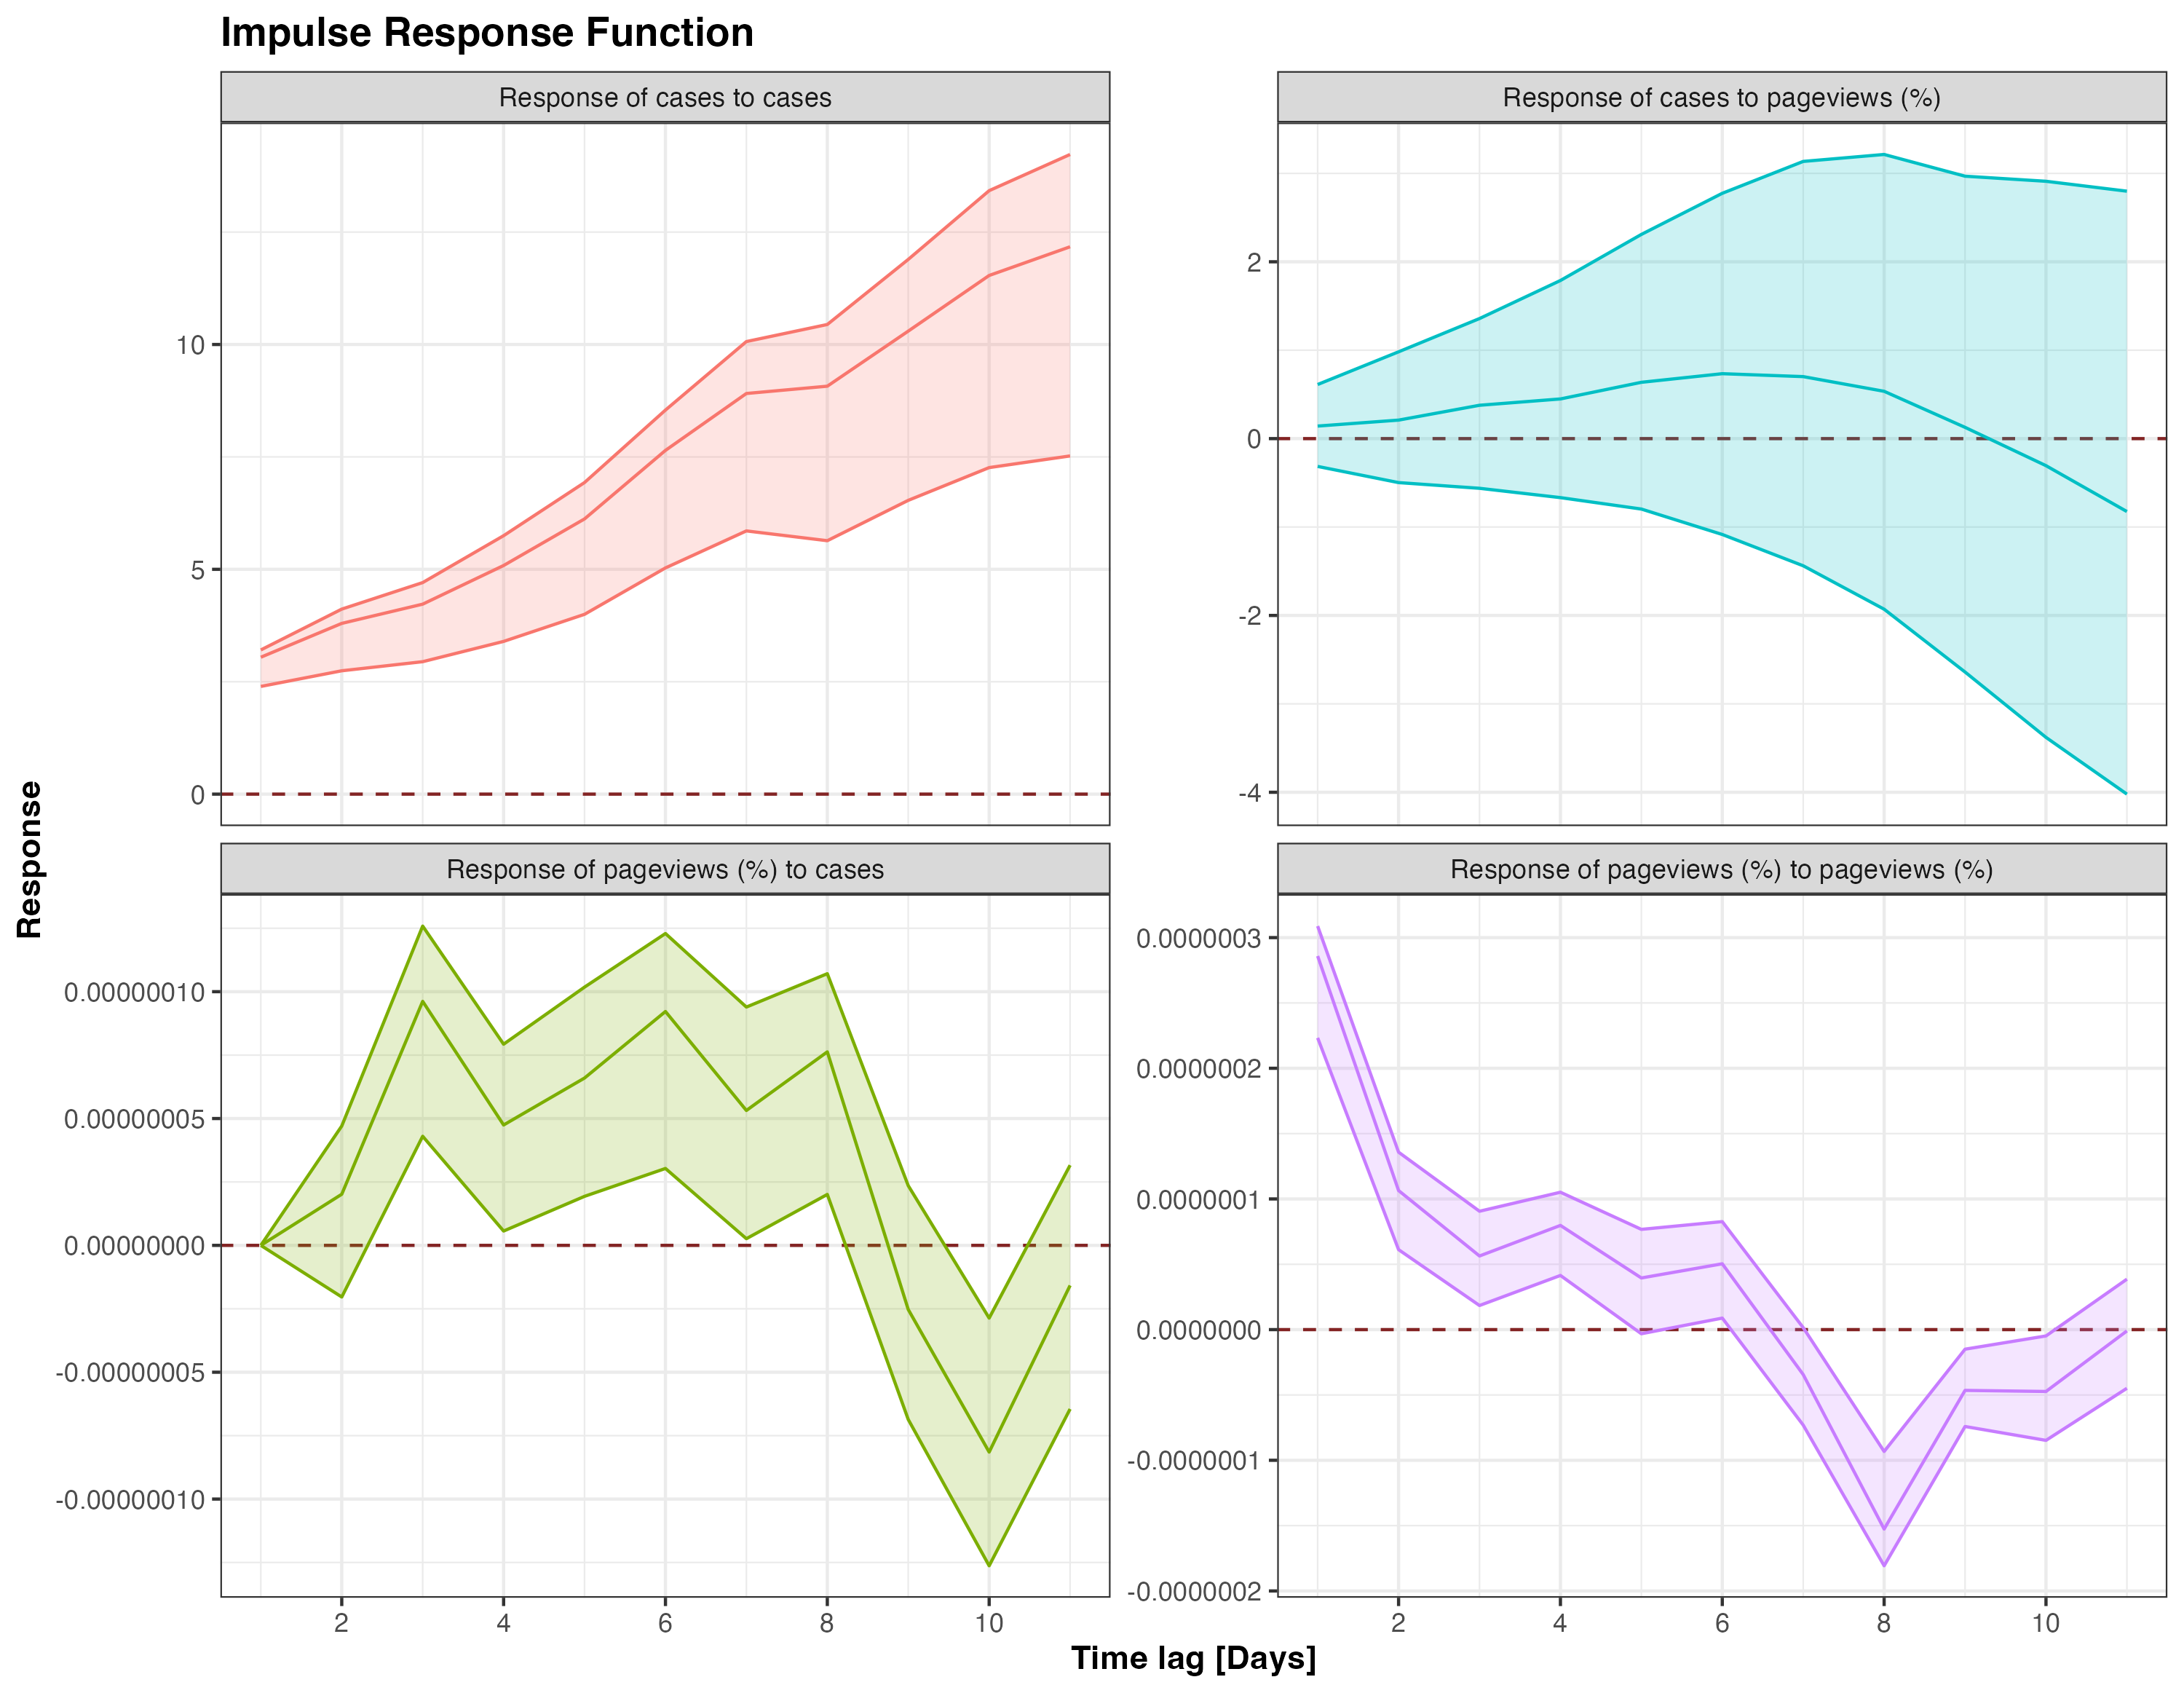
\includegraphics{images/impulse-response-function.png}

}

\caption{Impulse response function results}

\end{figure}%

The IRF analysis reveals the responses of mpox cases and pageviews to
shocks within each series, demonstrating how changes in one variable
affect the other over time. As observed from the plots, an initial shock
in mpox cases predicts a continual increase in subsequent cases over ten
days, indicating a potential compounding effect of cases on themselves.
Conversely, a shock in pageviews percentage forecasts a decreasing trend
in mpox cases over time, though with much uncertainty. The pageviews
percentage itself responds positively to a shock in mpox cases for about
eight days before declining, implying that case increases prompt a
temporary rise in public interest. Lastly, a surge in pageviews
percentage tends to peak quickly, followed by a recovery and then
another decline, potentially due to information saturation. The
confidence intervals across these graphs underscore the varying degrees
of certainty regarding these predictions.

The Granger-causality test results suggest a predictive relationship
between Wikipedia pageviews and mpox cases. The pageviews significantly
Granger-cause the number of cases (F-Test = 3.275, p-value \textless{}
0.001), indicating that changes in Wikipedia traffic can predict future
case numbers. Conversely, mpox cases also significantly Granger-cause
changes in pageviews (F-Test = 8.299, p-value \textless{} 0.001),
suggesting that the occurrence of cases can forecast subsequent online
search behavior. However, for both relationships, there is no evidence
of instantaneous causality, as indicated by the non-significant
Chi-squared statistic of 0.223 with a p-value of 0.637, implying that
neither variable instantaneously predicts changes in the other within
the same time frame.

\section{Discussion}\label{discussion}

\subsection{Key Findings}\label{key-findings}

There are several key findings from this analysis. First, the lag
analysis identifies several articles with significant Spearman time-lag
correlation for lags in which pageviews precede mpox cases, indicating
the potential predictive value of such articles. Furthermore, the
analysis reveals that the direction of correlation (positive or
negative) can vary depending on the time lag. This variability in
correlation suggests that the timing of information-seeking behavior on
Wikipedia is relevant and can both reflect and potentially anticipate
the rise or fall in mpox cases. Lastly, the different correlations
observed across articles emphasize the complexity of the relationship
between public information-seeking behavior and disease incidence. While
some search behaviors on Wikipedia follow the occurrence of cases,
others may serve as precursors, underscoring the bidirectional nature of
this relationship.

With regard to predictive modeling, none of the models provide a
consistently accurate representation across the entire timeline, with
difficulties in accurately capturing the peaks and troughs of outbreaks
and generalizing later time periods. This implies that while digital
traces like Wikipedia pageviews have potential in monitoring health
trends, there is a clear need for further refinement of predictive
models to ensure they are robust, generalizable, and accurate in diverse
scenarios. Furthermore, the inclusion of media coverage and scientific
interest appears to add some value to the models, providing a more
nuanced view of public interest and potentially improving predictions.
However, the enhancement is not substantial enough to align closely with
actual case trends, suggesting these factors alone are not sufficient
for accurate forecasts.

Utilizing a VAR model, there is evidence of a predictive relationship
between Wikipedia pageviews and mpox cases. The lagged data, which
accounted for up to 20 days prior, significantly influenced current
values, indicating that past data on pageviews and cases can inform
predictions of future trends. The IRF analysis demonstrated the dynamic
effect of shocks in one variable on the other. Shocks in mpox cases
predicted an increase in subsequent cases, while shocks in pageviews
indicated a potential decrease in future cases. Pageviews responded
positively to shocks in case numbers initially but settled back,
highlighting public attention patterns during health events. The
Granger-causality tests confirmed that Wikipedia pageviews and mpox
cases have a bidirectional predictive relationship, suggesting that
mpox-related pageviews can predict future case numbers and vice versa.
However, there was no evidence of instantaneous causality between the
two variables, suggesting the relationship unfolds over time rather than
simultaneously.

Overall, the analysis suggests that Wikipedia traffic can serve as a
valuable digital trace for monitoring and possibly forecasting public
health trends. However, the model's limitations, particularly concerning
the non-normality of residuals, serve as a reminder of the complexities
involved in using digital platforms for epidemiological surveillance and
the need for cautious interpretation of such models.

\subsection{Limitations}\label{limitations}

This paper identifies several limitations that could affect the
interpretation of the results and the generalizability of the findings.
While country-level Wikipedia pageview data provide several distinct
advantages, the dataset nevertheless comes with its own limitations.
Notably, the Wikimedia Foundation's approach to differential privacy
often results in significant data missingness, obscuring trends below
minimum pageview thresholds. Moreover, the data is~ disaggregated by
Wikipedia language version before the minimum pageview threshold is
applied, resulting in limited availability of pageview data for
linguistic minorities. While this is not a large concern in the context
of the United States where English represents approximately 90\% of
Wikipedia pageviews, this may not hold true in other contexts with
greater linguistic diversity, thereby limiting generalizability. On a
related note, the different minimum pageview thresholds applied to
countries depending on their Country and Territory Protection List
classifications, while of critical importance, does present a challenge
for implementing a uniform approach to disease modeling across different
countries. Additionally, it should be noted that country-level data is
available only from July 2015 onward, thereby limiting the scope for
retrospective analyses (\citeproc{ref-triedman2023}{Triedman and Ruiz
2023}). Lastly, demographic biases in Wikipedia's user base, which tend
to be younger, more educated, and male, may not accurately reflect the
broader public's concerns (\citeproc{ref-glott2010}{Glott and Ghosh
2010}). This skew could lead to misleading interpretations of public
interest in health issues.~

Methodologically, the study may not capture complex, nonlinear
interactions between Wikipedia pageviews and epidemiological trends
adequately. There's a notable risk of overfitting to specific case
studies like the 2022-2024 mpox outbreak, which could undermine the
findings' applicability to other diseases or contexts. Moreover, the
influence of exogenous factors such as media coverage and scientific
interest can significantly affect online search behaviors, complicating
the interpretation of online behavior as a direct reflection of public
health concerns~ (\citeproc{ref-eysenbach2011}{Eysenbach 2011}).
Additionally, the article selection process could also have been
expanded to include a broader range of health-related articles to
potentially identify other relevant articles for analysis.

\subsection{Future Research}\label{future-research}

Moving forward, there is considerable scope for refining these methods
to address these challenges. With regard to modeling, future work should
explore different combinations of predictors, employ regularization
techniques to prevent overfitting, and experiment with more
sophisticated statistical models that are better suited to non-linear
data or machine learning approaches. While this analysis specifically
examines the 2022-2024 mpox outbreak in the U.S. context, different
epidemiological events and time periods should be investigated to
explore the reliability and generalizability of findings across various
contexts. To account for the missingness common to country-level
Wikipedia pageview data, various imputation strategies should be
explored to better mitigate the impact of missing data as well as bias
potentially introduced by imputed values. Future work could also
quantify the extent to which different minimum pageview thresholds
impact the accuracy of predictive models when using county-level
Wikipedia pageview data. Finally, efforts should be made to de-noise the
data by more thoroughly investigating the impact that external
influences like media coverage and scientific interest have on
pageviews. This is important to address considering these factors often
skew public attention and complicate the interpretation of online
information-seeking behaviors, especially when driven by an ``epidemic
of fear'' (\citeproc{ref-eysenbach2011}{Eysenbach 2011}).

\subsection{Policy Recommendations}\label{policy-recommendations}

Based on the findings of this research, several actionable policy
recommendations can enhance public health strategies using open source
platforms such as Wikipedia. To improve the utility of the Wikimedia
Foundation's data for research and policymaking, it is suggested that
data release thresholds, which currently rely solely on a country's
classification under the Country and Territory Protection List, be
refined. Factors such as population size and internet usage rates should
be incorporated to allow for more detailed data availability, without
compromising privacy protections. To address concerns that lowering this
threshold could impact language minorities in countries, the Wikimedia
Foundation could aggregate pageviews by Wikidata ID. This is a unique
identifier that links different language versions of the same article.
This would have the potential to strengthen existing privacy
protections, while also potentially increasing the number of articles
with pageviews that exceed the minimum threshold.~

Public health officials should explore adopting these digital
epidemiological surveillance methods, incorporating them into existing
surveillance systems. It should be emphasized that these methods should
not replace traditional surveillance methods but rather supplement them.
While this paper specifically investigates the efficacy of Wikipedia,
other data sources should continue to be explored and used in
conjunction with one another, so as to achieve a more comprehensive view
of online health-related information-seeking behavior. By integrating
these methods into early warning systems against disease, more nuanced
public health interventions can be formulated, backed by empirical data
to mitigate the impacts of future outbreaks.

\subsection{Conclusion}\label{conclusion}

While leveraging digital traces of online health-related
information-seeking behavior to make case predictions is a difficult
endeavor, the elevated risk of widespread infectious disease outbreaks
driven by an increasingly interconnected global society and climate
change necessitates a careful examination of the digital tools
available. Harnessing internet-based data for disease surveillance has
the potential to enhance the speed and accuracy of public health
responses. By integrating real-time digital analytics into traditional
surveillance frameworks, public health agencies could significantly
improve their ability to predict and respond to emerging health threats.
Ultimately, this could lead to more proactive, rather than reactive,
approaches in managing public health crises, potentially saving
countless lives in the process.

\section*{References}\label{references}
\addcontentsline{toc}{section}{References}

\phantomsection\label{refs}
\begin{CSLReferences}{1}{0}
\bibitem[\citeproctext]{ref-abbas2021}
Abbas, Mostafa, Thomas B. Morland, Eric S. Hall, and Yasser
EL-Manzalawy. 2021. {``Associations Between Google Search Trends for
Symptoms and COVID-19 Confirmed and Death Cases in the United States.''}
\emph{International Journal of Environmental Research and Public Health}
18 (9): 4560. \url{https://doi.org/10.3390/ijerph18094560}.

\bibitem[\citeproctext]{ref-adawi2017}
Adawi, Mohammad, Nicola Luigi Bragazzi, Abdulla Watad, Kassem Sharif,
Howard Amital, and Naim Mahroum. 2017. {``Discrepancies Between Classic
and Digital Epidemiology in Searching for the Mayaro Virus: Preliminary
Qualitative and Quantitative Analysis of Google Trends.''} \emph{JMIR
Public Health and Surveillance} 3 (4): e9136.
\url{https://doi.org/10.2196/publichealth.9136}.

\bibitem[\citeproctext]{ref-arora2019}
Arora, Vishal S., Martin McKee, and David Stuckler. 2019. {``Google
Trends: Opportunities and limitations in health and health policy
research.''} \emph{Health Policy (Amsterdam, Netherlands)} 123 (3):
338--41. \url{https://doi.org/10.1016/j.healthpol.2019.01.001}.

\bibitem[\citeproctext]{ref-bao2013}
Bao, Jia-xing, Ben-fu Lv, Geng Peng, and Na Li. 2013. {``2013
International Conference on Management Science and Engineering 20th
Annual Conference Proceedings.''} In, 36--42.
\url{https://doi.org/10.1109/ICMSE.2013.6586259}.

\bibitem[\citeproctext]{ref-beer2019}
Beer, Ellen M., and V. Bhargavi Rao. 2019. {``A Systematic Review of the
Epidemiology of Human Monkeypox Outbreaks and Implications for Outbreak
Strategy.''} \emph{PLOS Neglected Tropical Diseases} 13 (10): e0007791.
\url{https://doi.org/10.1371/journal.pntd.0007791}.

\bibitem[\citeproctext]{ref-bernardo2013}
Bernardo, Theresa Marie, Andrijana Rajic, Ian Young, Katie Robiadek, Mai
T. Pham, and Julie A. Funk. 2013. {``Scoping Review on Search Queries
and Social Media for Disease Surveillance: A Chronology of
Innovation.''} \emph{Journal of Medical Internet Research} 15 (7):
e2740. \url{https://doi.org/10.2196/jmir.2740}.

\bibitem[\citeproctext]{ref-bragazzi2016}
Bragazzi, Nicola Luigi, Susanna Bacigaluppi, Chiara Robba, Anna Siri,
Giovanna Canepa, and Francesco Brigo. 2016. {``Infodemiological Data of
West-Nile Virus Disease in Italy in the Study Period
2004{\textendash}2015.''} \emph{Data in Brief} 9 (December): 839--45.
\url{https://doi.org/10.1016/j.dib.2016.10.022}.

\bibitem[\citeproctext]{ref-brownstein2009}
Brownstein, John S., Clark C. Freifeld, and Lawrence C. Madoff. 2009.
{``Digital Disease Detection {\textemdash} Harnessing the Web for Public
Health Surveillance.''} \emph{The New England Journal of Medicine} 360
(21): 2153--57. \url{https://doi.org/10.1056/NEJMp0900702}.

\bibitem[\citeproctext]{ref-butler2013}
Butler, Declan. 2013. {``When Google Got Flu Wrong.''} \emph{Nature} 494
(7436): 155--56. \url{https://doi.org/10.1038/494155a}.

\bibitem[\citeproctext]{ref-cdc2023}
CDC. 2023. {``Mpox in the u.s.''}
\url{https://www.cdc.gov/poxvirus/mpox/response/2022/mpx-trends.html}.

\bibitem[\citeproctext]{ref-cdcmap}
---------. 2024. {``2022-2023 u.s. Map \& Case Count.''}
\url{https://www.cdc.gov/poxvirus/mpox/response/2022/us-map.html}.

\bibitem[\citeproctext]{ref-cervellin2017}
Cervellin, Gianfranco, Ivan Comelli, and Giuseppe Lippi. 2017. {``Is
Google Trends a reliable tool for digital epidemiology? Insights from
different clinical settings.''} \emph{Journal of Epidemiology and Global
Health} 7 (3): 185--89.
\url{https://doi.org/10.1016/j.jegh.2017.06.001}.

\bibitem[\citeproctext]{ref-chrzanowski2021}
Chrzanowski, Jędrzej, Julia Sołek, Wojciech Fendler, and Dariusz
Jemielniak. 2021. {``Assessing Public Interest Based on Wikipedia{'}s
Most Visited Medical Articles During the SARS-CoV-2 Outbreak: Search
Trends Analysis.''} \emph{Journal of Medical Internet Research} 23 (4).
\url{https://doi.org/10.2196/26331}.

\bibitem[\citeproctext]{ref-downs}
Downs, Anthony. 1972. {``Up and Down with Ecology - the 'Issue-Attention
Cycle'.''} \emph{The Public Interest}.

\bibitem[\citeproctext]{ref-du2023}
Du, Min, Chenyuan Qin, Wenxin Yan, Qiao Liu, Yaping Wang, Lin Zhu,
Wannian Liang, Min Liu, and Jue Liu. 2023. {``Trends in Online Search
Activity and the Correlation with Daily New Cases of Monkeypox Among 102
Countries or Territories.''} \emph{International Journal of
Environmental Research and Public Health} 20 (4).
\url{https://doi.org/10.3390/ijerph20043395}.

\bibitem[\citeproctext]{ref-effenberger2020}
Effenberger, Maria, Andreas Kronbichler, Jae Il Shin, Gert Mayer,
Herbert Tilg, and Paul Perco. 2020. {``Association of the COVID-19
pandemic with Internet Search Volumes: A Google TrendsTM Analysis.''}
\emph{International journal of infectious diseases: IJID: official
publication of the International Society for Infectious Diseases} 95
(June): 192--97. \url{https://doi.org/10.1016/j.ijid.2020.04.033}.

\bibitem[\citeproctext]{ref-eysenbach2011}
Eysenbach, Gunther. 2011. {``Infodemiology and Infoveillance: Tracking
Online Health Information and Cyberbehavior for Public Health.''}
\emph{American Journal of Preventive Medicine} 40 (5): S154--58.
\url{https://doi.org/10.1016/j.amepre.2011.02.006}.

\bibitem[\citeproctext]{ref-generous2014}
Generous, Nicholas, Geoffrey Fairchild, Alina Deshpande, Sara Y. Del
Valle, and Reid Priedhorsky. 2014. {``Global Disease Monitoring and
Forecasting with Wikipedia.''} \emph{PLOS Computational Biology} 10
(11): e1003892. \url{https://doi.org/10.1371/journal.pcbi.1003892}.

\bibitem[\citeproctext]{ref-gessainantoine2022}
Gessain, Antoine, Emmanuel Nakoune, and Yazdan Yazdanpanah. 2022.
{``Monkeypox.''} \emph{New England Journal of Medicine} 387 (19):
1783--93. \url{https://doi.org/10.1056/NEJMra2208860}.

\bibitem[\citeproctext]{ref-ginsberg2009}
Ginsberg, Jeremy, Matthew H. Mohebbi, Rajan S. Patel, Lynnette Brammer,
Mark S. Smolinski, and Larry Brilliant. 2009. {``Detecting Influenza
Epidemics Using Search Engine Query Data.''} \emph{Nature} 457 (7232):
1012--14. \url{https://doi.org/10.1038/nature07634}.

\bibitem[\citeproctext]{ref-glott2010}
Glott, Ruediger, and Rishab Ghosh. 2010. {``Topic: Age and Gender
Differences.''}

\bibitem[\citeproctext]{ref-gnewsap}
{``GNews API: Your Gateway to the Power of News APIs.''} 2024.
\url{https://gnews.io/}.

\bibitem[\citeproctext]{ref-gong2022}
Gong, Xue, Mengchi Hou, Yangyang Han, Hailun Liang, and Rui Guo. 2022.
{``Application of the Internet Platform in Monitoring Chinese Public
Attention to the Outbreak of COVID-19.''} \emph{Frontiers in Public
Health} 9 (January): 755530.
\url{https://doi.org/10.3389/fpubh.2021.755530}.

\bibitem[\citeproctext]{ref-gozzi2020}
Gozzi, N., Michele Tizzani, Michele Starnini, F. Ciulla, D. Paolotti, A.
Panisson, and N. Perra. 2020. {``Collective Response to the Media
Coverage of COVID-19 Pandemic on Reddit and Wikipedia.''} \emph{ArXiv},
June.
\url{https://www.semanticscholar.org/paper/b6e8ffbcb91c70ea9688676135228b4cb1173883}.

\bibitem[\citeproctext]{ref-hickmann2015}
Hickmann, Kyle S., Geoffrey Fairchild, Reid Priedhorsky, Nicholas
Generous, James M. Hyman, Alina Deshpande, and Sara Y. Del Valle. 2015.
{``Forecasting the 2013{\textendash}2014 Influenza Season Using
Wikipedia.''} \emph{PLOS Computational Biology} 11 (5): e1004239.
\url{https://doi.org/10.1371/journal.pcbi.1004239}.

\bibitem[\citeproctext]{ref-james2016}
James, Richard. 2016. {``WikiProject Medicine: Creating Credibility in
Consumer Health.''} \emph{Journal of Hospital Librarianship} 16 (4):
344351. \url{https://doi.org/10.1080/15323269.2016.1221284}.

\bibitem[\citeproctext]{ref-kuxe4mpf2015}
Kämpf, Mirko, Eric Tessenow, Dror Y. Kenett, and Jan W. Kantelhardt.
2015. {``The Detection of Emerging Trends Using Wikipedia Traffic Data
and Context Networks.''} \emph{PloS One} 10 (12): e0141892.
\url{https://doi.org/10.1371/journal.pone.0141892}.

\bibitem[\citeproctext]{ref-wikipedir}
Keyes, Os, Brock Tilber, and Clemens Schmid. 2024. {``Package
{`WikipediR'}: A MediaWiki API Wrapper.''}
\url{https://cran.r-project.org/web/packages/WikipediR/WikipediR.pdf}.

\bibitem[\citeproctext]{ref-kman2012}
Kman, Nicholas E., and Daniel J. Bachmann. 2012. {``Biosurveillance: a
review and update.''} \emph{Advances in Preventive Medicine} 2012:
301408. \url{https://doi.org/10.1155/2012/301408}.

\bibitem[\citeproctext]{ref-laurenson-schafer2023}
Laurenson-Schafer, Henry, Nikola Sklenovská, Ana Hoxha, Steven M. Kerr,
Patricia Ndumbi, Julia Fitzner, Maria Almiron, et al. 2023.
{``Description of the First Global Outbreak of Mpox: An Analysis of
Global Surveillance Data.''} \emph{The Lancet Global Health} 11 (7):
e1012--23. \url{https://doi.org/10.1016/S2214-109X(23)00198-5}.

\bibitem[\citeproctext]{ref-laurent2009}
Laurent, Michaël R, and Tim J Vickers. 2009. {``Seeking health
information online: does Wikipedia matter.''} \emph{Journal of the
American Medical Informatics Association} 16 (4): 471--79.
\url{https://doi.org/10.1197/jamia.m3059}.

\bibitem[\citeproctext]{ref-lazer2014}
Lazer, David, Ryan Kennedy, Gary King, and Alessandro Vespignani. 2014.
{``The Parable of Google Flu: Traps in Big Data Analysis.''}
\emph{Science} 343 (6176): 1203--5.
\url{https://doi.org/10.1126/science.1248506}.

\bibitem[\citeproctext]{ref-liu2022}
Liu, Yang, Zhiying Yue, and Mohd Anwar. 2022. {``2022 IEEE/ACM
Conference on Connected Health: Applications, Systems and Engineering
Technologies (CHASE).''} In, 166--67.
\url{https://ieeexplore.ieee.org/document/9983632}.

\bibitem[\citeproctext]{ref-marques-toledo2017}
Marques-Toledo, Cecilia de Almeida, Carolin Marlen Degener, Livia
Vinhal, Giovanini Coelho, Wagner Meira, Claudia Torres Codeço, and Mauro
Martins Teixeira. 2017. {``Dengue Prediction by the Web: Tweets Are a
Useful Tool for Estimating and Forecasting Dengue at Country and City
Level.''} \emph{PLOS Neglected Tropical Diseases} 11 (7): e0005729.
\url{https://doi.org/10.1371/journal.pntd.0005729}.

\bibitem[\citeproctext]{ref-mciver2014}
McIver, David J., and John S. Brownstein. 2014. {``Wikipedia Usage
Estimates Prevalence of Influenza-Like Illness in the United States in
Near Real-Time.''} \emph{PLOS Computational Biology} 10 (4): e1003581.
\url{https://doi.org/10.1371/journal.pcbi.1003581}.

\bibitem[\citeproctext]{ref-mcquiston2023}
McQuiston, Jennifer H. 2023. {``The CDC Domestic Mpox Response
{\textemdash} United States, 2022{\textendash}2023.''} \emph{MMWR.
Morbidity and Mortality Weekly Report} 72.
\url{https://doi.org/10.15585/mmwr.mm7220a2}.

\bibitem[\citeproctext]{ref-getstar}
Meta. 2022. {``Get Started with the Page Insights API.''}
\url{https://developers.facebook.com/blog/post/2022/11/08/getting-started-with-page-insights-api/}.

\bibitem[\citeproctext]{ref-munzert}
Munzert. 2015. {``Using Wikipedia Article Traffic Volume to Measure
Public Issue Attention - Work in Progress.''}
\url{https://github.com/simonmunzert/workingPapers/blob/master/wikipedia-salience-v3.pdf}.

\bibitem[\citeproctext]{ref-ocampo2013}
Ocampo, Alex J., Rumi Chunara, and John S. Brownstein. 2013. {``Using
Search Queries for Malaria Surveillance, Thailand.''} \emph{Malaria
Journal} 12 (1): 390. \url{https://doi.org/10.1186/1475-2875-12-390}.

\bibitem[\citeproctext]{ref-olson2013}
Olson, Donald R., Kevin J. Konty, Marc Paladini, Cecile Viboud, and Lone
Simonsen. 2013. {``Reassessing Google Flu Trends data for detection of
seasonal and pandemic influenza: a comparative epidemiological study at
three geographic scales.''} \emph{PLoS computational biology} 9 (10):
e1003256. \url{https://doi.org/10.1371/journal.pcbi.1003256}.

\bibitem[\citeproctext]{ref-pageview}
{``Pageviews Differential Privacy {\textemdash} Current.''} n.d.
\url{https://analytics.wikimedia.org/published/datasets/country_project_page/00_README.html}.

\bibitem[\citeproctext]{ref-pageviewhist}
{``Pageviews Differential Privacy {\textemdash} Historical.''} n.d.
\url{https://analytics.wikimedia.org/published/datasets/country_project_page_historical/00_README.html}.

\bibitem[\citeproctext]{ref-paul2011}
Paul, Michael, and Mark Dredze. 2011. {``You Are What You Tweet:
Analyzing Twitter for Public Health.''} \emph{Proceedings of the
International AAAI Conference on Web and Social Media} 5 (1): 265--72.
\url{https://doi.org/10.1609/icwsm.v5i1.14137}.

\bibitem[\citeproctext]{ref-polgreen2008}
Polgreen, Philip M., Yiling Chen, David M. Pennock, Forrest D. Nelson,
and Robert A. Weinstein. 2008. {``Using Internet Searches for Influenza
Surveillance.''} \emph{Clinical Infectious Diseases} 47 (11): 1443--48.
\url{https://doi.org/10.1086/593098}.

\bibitem[\citeproctext]{ref-romanello2021}
Romanello, Marina, Alice McGushin, Claudia Di Napoli, Paul Drummond,
Nick Hughes, Louis Jamart, Harry Kennard, et al. 2021. {``The 2021
Report of the Lancet Countdown on Health and Climate Change: Code Red
for a Healthy Future.''} \emph{The Lancet} 398 (10311): 1619--62.
\url{https://doi.org/10.1016/S0140-6736(21)01787-6}.

\bibitem[\citeproctext]{ref-schober2020}
Schober, Patrick, and Thomas R. Vetter. 2020. {``Correlation Analysis in
Medical Research.''} \emph{Anesthesia and Analgesia} 130 (2): 332.
\url{https://doi.org/10.1213/ANE.0000000000004578}.

\bibitem[\citeproctext]{ref-topwebs}
Semrush. 2024. {``Top Websites in the World - March 2024 Most Visited \&
Popular Rankings.''} \url{https://www.semrush.com/website/top/}.

\bibitem[\citeproctext]{ref-sousa-pinto2020}
Sousa-Pinto, Bernardo, Aram Anto, Wienia Czarlewski, Josep M. Anto, João
Almeida Fonseca, and Jean Bousquet. 2020. {``Assessment of the Impact of
Media Coverage on COVID-19{\textendash}Related Google Trends Data:
Infodemiology Study.''} \emph{Journal of Medical Internet Research} 22
(8): e19611. \url{https://doi.org/10.2196/19611}.

\bibitem[\citeproctext]{ref-rformac}
Statistical Computing, R Foundation for. 2024. {``R Version 4.3.3
(2024-02-29) -- "Angel Food Cake".''} \url{https://cran.r-project.org/}.

\bibitem[\citeproctext]{ref-tausczik2012}
Tausczik, Yla, Kate Faasse, James W. Pennebaker, and Keith J. Petrie.
2012. {``Public Anxiety and Information Seeking Following the H1N1
Outbreak: Blogs, Newspaper Articles, and Wikipedia Visits.''}
\emph{Health Communication} 27 (2): 179185.
\url{https://doi.org/10.1080/10410236.2011.571759}.

\bibitem[\citeproctext]{ref-triedman2023}
Triedman, Hal, and Isaac Johnsonand Nuria Ruiz. 2023. {``New Dataset
Uncovers Wikipedia Browsing Habits While Protecting Users.''}
\url{https://diff.wikimedia.org/2023/06/21/new-dataset-uncovers-wikipedia-browsing-habits-while-protecting-users/}.

\bibitem[\citeproctext]{ref-secondm}
WHO. 2022a. {``Second Meeting of the International Health Regulations
(2005) (IHR) Emergency Committee Regarding the Multi-Country Outbreak of
Monkeypox.''}
\url{https://www.who.int/news/item/23-07-2022-second-meeting-of-the-international-health-regulations-(2005)-(ihr)-emergency-committee-regarding-the-multi-country-outbreak-of-monkeypox}.

\bibitem[\citeproctext]{ref-whodire}
---------. 2022b. {``WHO Director-General's Statement at the Press
Conference Following IHR Emergency Committee Regarding the Multi-Country
Outbreak of Monkeypox - 23 July 2022.''}
\url{https://www.who.int/director-general/speeches/detail/who-director-general-s-statement-on-the-press-conference-following-IHR-emergency-committee-regarding-the-multi--country-outbreak-of-monkeypox--23-july-2022}.

\bibitem[\citeproctext]{ref-whoreco}
---------. 2022c. {``WHO Recommends New Name for Monkeypox Disease.''}
\url{https://www.who.int/news/item/28-11-2022-who-recommends-new-name-for-monkeypox-disease}.

\bibitem[\citeproctext]{ref-worldhealthorganization}
---------. 2023a. {``Mpox (Monkeypox).''}
\url{https://www.who.int/news-room/fact-sheets/detail/monkeypox}.

\bibitem[\citeproctext]{ref-mpox_cif}
---------. 2023b. {``Mpox (Monkeypox) Case Investigation Form (CIF) and
Minimum Dataset Case Reporting Form (CRF).''}
\url{https://www.who.int/publications/m/item/monkeypox-minimum-dataset-case-reporting-form-(crf)}.

\bibitem[\citeproctext]{ref-fifthme}
---------. 2023c. {``Fifth Meeting of the International Health
Regulations (2005) (IHR) Emergency Committee on the Multi-Country
Outbreak of Mpox (Monkeypox).''}
\url{https://www.who.int/news/item/11-05-2023-fifth-meeting-of-the-international-health-regulations-(2005)-(ihr)-emergency-committee-on-the-multi-country-outbreak-of-monkeypox-(mpox)}.

\bibitem[\citeproctext]{ref-whoshiny}
---------. 2024. {``2022-24 Mpox Outbreak: Global Trends.''}
\url{https://worldhealthorg.shinyapps.io/mpx_global}.

\bibitem[\citeproctext]{ref-wikimediafoundation}
Wikimedia Statistics. 2024. {``Wikimedia Statistics - All Wikipedias.''}
\url{https://stats.wikimedia.org/\#/all-wikipedia-projects}.

\bibitem[\citeproctext]{ref-wikimedi}
{``Wikimedia Traffic Analysis Report - Page Views Per Wikipedia Language
- Breakdown.''} n.d.
\url{https://stats.wikimedia.org/wikimedia/squids/SquidReportPageViewsPerLanguageBreakdown.htm}.

\bibitem[\citeproctext]{ref-wikimediafoundation2024}
Wikipedia. 2024a. {``WikiProject Medicine.''}
\url{https://en.wikipedia.org/w/index.php?title=Wikipedia:WikiProject_Medicine&oldid=1209391449}.

\bibitem[\citeproctext]{ref-wikipedi2024}
---------. 2024b. {``Size of Wikipedia.''}
\url{https://en.wikipedia.org/w/index.php?title=Wikipedia:Size_of_Wikipedia&oldid=1216603163}.

\bibitem[\citeproctext]{ref-winter2020}
Winter, David, Scott Chamberlain, and Han Guangchun. 2020.
\emph{Rentrez: 'Entrez' in r}.
\url{https://cran.r-project.org/web/packages/rentrez/index.html}.

\bibitem[\citeproctext]{ref-xapi}
X. 2024. {``API Products.''}
\url{https://developer.twitter.com/en/products/twitter-api}.

\bibitem[\citeproctext]{ref-yan2023}
Yan, Wenxin, Min Du, Chenyuan Qin, Qiao Liu, Yaping Wang, Wannian Liang,
Min Liu, and Jue Liu. 2023. {``Association Between Public Attention and
Monkeypox Epidemic: A Global Lag{-}Correlation Analysis.''}
\emph{Journal of Medical Virology} 95 (1): e28382.
\url{https://doi.org/10.1002/jmv.28382}.

\bibitem[\citeproctext]{ref-yang2011}
Yang, Albert C., Shi-Jen Tsai, Norden E. Huang, and Chung-Kang Peng.
2011. {``Association of Internet Search Trends with Suicide Death in
Taipei City, Taiwan, 2004{\textendash}2009.''} \emph{Journal of
Affective Disorders} 132 (1): 179--84.
\url{https://doi.org/10.1016/j.jad.2011.01.019}.

\bibitem[\citeproctext]{ref-yuan2021}
Yuan, Kai, Guangrui Huang, Lepeng Wang, Ting Wang, Wenbin Liu, Haixu
Jiang, and Albert C. Yang. 2021. {``Predicting Norovirus in the United
States Using Google Trends: Infodemiology Study.''} \emph{Journal of
Medical Internet Research} 23 (9): e24554.
\url{https://doi.org/10.2196/24554}.

\bibitem[\citeproctext]{ref-yuan2013}
Yuan, Qingyu, Elaine O. Nsoesie, Benfu Lv, Geng Peng, Rumi Chunara, and
John S. Brownstein. 2013. {``Monitoring influenza epidemics in china
with search query from baidu.''} \emph{PloS One} 8 (5): e64323.
\url{https://doi.org/10.1371/journal.pone.0064323}.

\bibitem[\citeproctext]{ref-zhou2010}
Zhou, Xi-chuan, and Hai-bin Shen. 2010. {``Notifiable Infectious Disease
Surveillance with Data Collected by Search Engine.''} \emph{Journal of
Zhejiang University SCIENCE C} 11 (4): 241--48.
\url{https://doi.org/10.1631/jzus.C0910371}.

\end{CSLReferences}



\end{document}
